% Created 2015-12-13 Sun 11:26
\documentclass[graduation-thesis]{mlarticle}
     \usepackage[dvipdfmx]{graphicx}
     \usepackage{url}
     \usepackage{atbegshi}
     \AtBeginShipoutFirst{\special{pdf:tounicode EUC-UCS2}}
     \usepackage[dvipdfmx,setpagesize=false]{hyperref}
          \usepackage[dvipdfmx]{color}
\usepackage{url}
\usepackage{float}
\usepackage[setpagesize=false]{hyperref}
\usepackage{ascmac}
\usepackage{here}
\usepackage{txfonts}
\usepackage{listings, jlisting}
\author{61200185 情報工学科 縣直道}
\date{\today}
\title{}
\begin{document}


\makeatletter
\renewcommand{\thetable}{
        \thesection.\arabic{table}
} %「表(章番号)-#.」と表記するための措置
\@addtoreset{table}{section}
  
\renewcommand{\thefigure}{
        \thesection.\arabic{figure}
}
\@addtoreset{figure}{section} %「図(章番号)-#.」と表記するための措置

\setcounter{page}{1}

\pagenumbering{roman}
\tableofcontents
\clearpage

\pagenumbering{arabic}

\definecolor{keywords}{RGB}{255,0,90}
\definecolor{comments}{RGB}{0,0,113}
\definecolor{red}{RGB}{160,0,0}
\definecolor{green}{RGB}{0,150,0}
 
\lstset{
        basicstyle=\ttfamily\footnotesize, 
        frame=single,
        keywordstyle=\color{keywords},
        commentstyle=\color{comments},
        stringstyle=\color{red},
        showstringspaces=false,
        identifierstyle=\color{green},
        }
\section{はじめに}
\label{intro}
\subsection {背景}
\label {intro:background}
現在,仮想化技術が普及してきており,様々なサービスの基盤技術として広く用いられている.
仮想化技術の利用例として,クラウドコンピューティングやInfrastructure as a Service (IaaS) が挙げられる.
物理マシンという限られたリソースを仮想化することで,複数の利用者が安全にリソースを共有することが可能となる.
IaaS は仮想化されたコンピュータ基盤をインターネット経由でサービスとして提供するものである.

クラウド環境上では,一台の仮想マシン上で,一つのアプリケーションのみを実行する場合がほとんどである.
これは,クラウド環境上では,物理マシンというリソースを増やすことなく仮想マシンを増やすことが可能であり,複数のアプリケーションを実行する場合には仮想マシンを増やすことで対処可能なためである.

このようなクラウド環境上の仮想マシンには,ほとんどの場合,物理マシン上で利用されるような汎用オペレーティングシステム(Linux,Windows,*BSD)が利用される.

\subsection {問題点}
\label {intro:problem}
汎用オペレーティングシステムは,高度な抽象化,機能を多数備えている.
オペレーティングシステム上で動作するアプリケーションが固定されている場合,それらの抽象化,機能は不要となる.

クラウド環境上の仮想マシンでは,ほとんどの場合,動作するアプリケーションが固定されている.
仮想マシンに汎用オペレーティングシステムを利用する場合,使用されることのないオペレーティングシステムの機能のために,カーネルイメージのサイズが増大し,セキュリティにも問題を抱えることになる. 
カーネルイメージのサイズが大きいと仮想マシンのサイズも大きくなり,仮想マシンの起動時間も大きくなる.
クラウド環境では,一つのアプリケーションごとに一台の仮想マシンを立ち上げるため,これらは大きな問題となる.

この問題の解決案として,あるアプリケーションに特化したオペレーティングシステムを開発するという方法が考えられる.
しかし,この方法は現実的とは言えない.オペレーティングシステムの開発は難しく,誤った実装が行われた場合システム全体に影響を及ぼしてしまう.
さらに,アプリケーションごとに新たにオペレーティングシステムを開発する必要があるという問題もある.

\subsection {提案}
\label{intro:proposal}
本研究では,汎用オペレーティングシステムから,アプリケーションが必要としない機能を自動的に削除することで,アプリケーションに特化したカーネルを生成する.
アプリケーションのソースコードを静的解析することで,必要となるオペレーティングシステムの機能を絞り込み,ブートに必要な部分と絞り込んだ機能を実装している部分のみを残すよう,カーネルのソースコードを書き換える.
自動的にカーネルを改変することで,アプリケーションごとに特化したオペレーティングシステムを開発する必要があるという問題点を解決する.

\subsection {実装}
\label{intro:implementation}
% TODO: gcov と openstack のリファレンス
まず,Linux カーネルソースコードの内,ブートに必要な部分とそうでない部分を分類する必要がある.
アプリケーションが使用する機能以外のすべてのソースコードを削除してしまうとブートすることが出来ないオペレーティングシステムになってしまう.
本研究では,この分類を行う手法を実装した.

本研究では,ブートに必要な部分を判別するため,gcov を用い,ブートまでのコードカバレッジを取得した.
ここから,ブートまでに一度も実行されていなかった関数を判別することができる.

ブートまでに一度も実行されていなかった関数をすべて削除したカーネルはブートすることが出来なかったため,Open Stack 上でカーネルがブートすることをテストできる環境を構築し,現在実験中である.

\subsection {論文の構成}
\label{intro:arch}
本論文の構成をいかに示す.
第\ref{relative}章では,本研究と関連する研究を紹介する.

\section {関連研究}
\label{relative}

本章では,本研究と関連する研究を紹介する.
Exokernel は,極小さなカーネルに,ライブラリとして高度な機能を付加する構成を提案している.
OSv は,仮想マシン上で一つのアプリケーションのみを実行する環境に特化したオペレーティングシステムを開発した.
Unikernel は,カーネルコンパイル時に,オペレーティングシステムの機能の有無を設定することができるカーネルである.

\subsection {Exokernel: An Operating System Architecture for Application-Level Resource Management}
\label{ralarive:exokernel}
カーネルのサイズを小さくするために,極単純な機能のみを持つカーネルに,Library OS として高レベルな抽象化などの機能を付加するという構成を提案している.

中心となる極小さなカーネルは,ハードウェア資源にアクセスするための低レベルなインターフェースを提供する役割のみを持つ.
プロセス,ファイル,アドレス空間,プロセス間通信といった高レベルな抽象化は,カーネルの提供するインターフェースを用いて,すべてカーネル外のライブラリとして実装される.
このような構成にすることで,アプリケーションが必要とする抽象化のみを提供することができ,アプリケーションが直接ハードウェア資源にアクセスすることも可能となる.
また,アプリケーションが必要とする機能のみをもつオペレーティングシステムを構築できるため,オペレーティングシステムによるオーバヘッドやメモリ使用量の増加といった問題を解決することができる.

% TODO: Exokernel の本研究との関連をうまく説明

Exokernel の構成では,アプリケーションを変えると,そのアプリケーションが必要とする抽象化を選択し再構成する必要が生じる.

\subsection {OSv - Optimizing the Operating System for Virtual Machines}

====================





現在,仮想化技術が様々なサービスを提供するための基盤技術として用いられている.
例えば,クラウドコンピューティングにおいても仮想化技術が用いられており,
ネットワークを介してアプリケーションを稼働させるためのプラットフォームを
ユーザに提供する PaaS は図\ref{paas} のように予め環境を構築してある
仮想マシンを提供することで実現されている.
よってユーザに提供されるプラットフォームはユーザに対して実際に一台の実機が用意されているわけではなく,
一人のユーザに一台の仮想マシンが用意されており,その仮想マシンがユーザに提供されている.
ユーザは PaaS によって環境構築の手間が省け,使用する資源の量を柔軟に変更することできる.
仮想化技術で構築された環境の管理には Live Migration が用いられる.
Live Migration とは仮想マシンを稼働したまま他の物理マシンに移送する技術である.
Live Migration を利用すると仮想マシンを稼働したまま移送できることから負荷分散,
マシンメンテナンス,省電力などにおいて有用である.
例えば,単体の物理マシン上で各仮想マシンの負荷総量が過剰になった時に負荷分散のために
一部の仮想マシンを他の物理マシンへ待避する

\begin{figure}[H]\begin{center}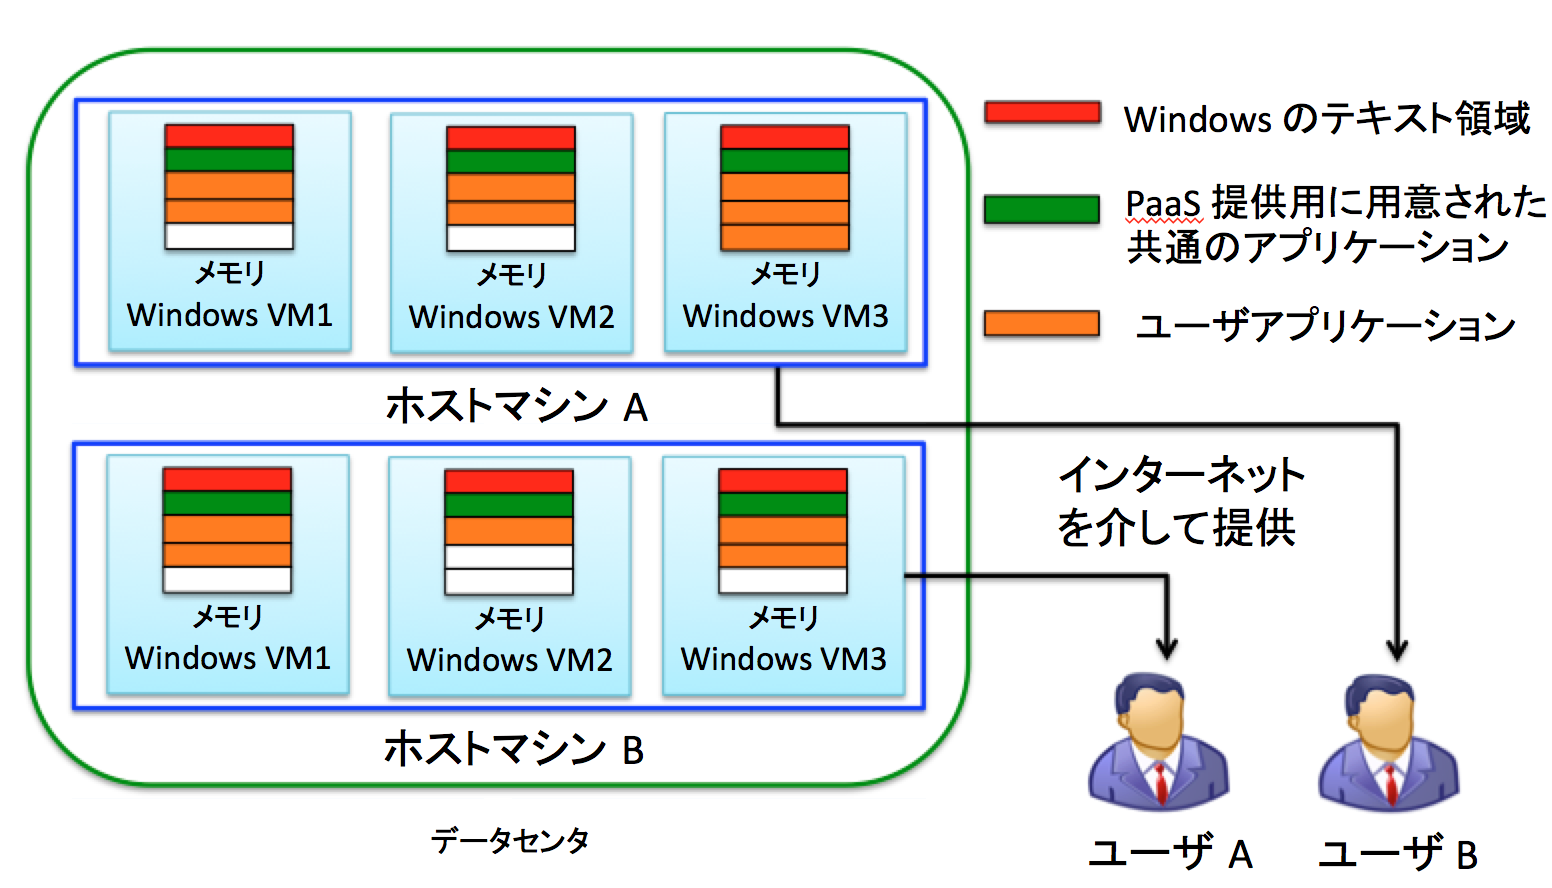
\includegraphics[width=10.0cm]{./img/paas.png}\caption{ PaaS 環境の例}\label{paas}\end{center}\end{figure}

既存の Live Migration では仮想マシンの全てのメモリを異なる物理マシン上に送信するため
メモリの送信総量が大きい.
Live Migration に必要な時間の大半はメモリ送信であるため,
メモリ移送量が多い程移送時間が長くなる.同時にネットワーク資源も移送量が多い程多く使用することになる.
ネットワーク資源の圧迫は他の仮想マシンにも影響を与える場合がある.
他にも,Live Migration は多くの CPU を使用するため,
この場合も移送する仮想マシン以外の仮想マシンに影響を与える場合がある\cite{Koto:2012:TUV}.
例えば,仮想マシンの負荷分散のために Live Migration を使用するときに
移送時間が長いことから高負荷なワークロードに追従することができず負荷分散が行えない場合がある.

そこで PaaS 環境における Live Migration で,移送する仮想マシンのメモリと同様のメモリが移送先物理マシンに
あるときはそのメモリは移送せず,移送先で共有し再利用する ShringMigration を提案する.
図\ref{paas} の VM1 をホストマシン A からホストマシン B へ移送するような場合を考えたとき
PaaS のような環境では移送する仮想マシンと同じ内容のメモリを
持つ仮想マシンが移送先にある場合が通常の仮想化環境より多くなる.
その場合,移送する仮想マシンの同じメモリページは移送先で再利用可能なので,
そのメモリページは移送せず移送先で共有し再利用することが可能である.
移送メモリの総量を減らすことで移送時間を短くし,使用ネットワーク量も減らす.
移送時間を短くすることで CPU の使用率も削減する.
また資源の使用を削減することで,移送する仮想マシン以外の仮想マシンへの影響を軽減する.

実験では既存の Live Migration より提案手法の Live Migration の方が移送時間を最大 37\% 削減する
ことができた.移送時間を短くすることでネットワークと CPU の使用量が少なくすることができる.

\clearpage
\section{仮想化技術}
\label{sec-2}
現在仮想化技術は様々なサービス提供の基盤技術として使用されている.
本章では仮想化技術全般の話や,クラウドコンピューティングにおける仮想化技術,
Live Migration ,仮想マシンのページ共有技術について説明する.
\subsection{仮想化}
\label{sec-2-1}
\subsubsection{仮想化とは}
\label{sec-2-1-1}
現在 IT の複雑さが増しており,取り扱いも比例して複雑化している.そのような技術を簡単で扱いやすい
ものにするのが仮想化の根本的な考え方である.つまり IT における仮想化とは
「ストレージ,メモリなどの計算資源の複雑な技術特性を隠蔽し,論理的な利用単位にし提供する技術」
と考えることができる.その利用単位の粒度によって仮想化は様々な種類にわけられる.
粒度の小さい例で言えばマルチプロセッサがあげられる.これは CPU を仮想化する技術で,
物理的には一つしかない CPU を時間単位などで使用を分配することであたかも複数の CPU が
動作しているように振舞わせる技術である.大きな粒度で見ればサーバのクラスタリング技術などがあげられる.
クラスタリング技術とは複数のコンピュータを繋げて,クライアントには1台のコンピュータだけが動作している
かのように振る舞わせる技術である.また物理リソースの特性を隠蔽し,ユーザにサービスを提供する
OS も仮想化といえる.
\subsubsection{サーバ仮想化}
\label{sec-2-1-2}
IT システムでは色々な仮想化技術が使用されている.その仮想化技術のひとつとして
サーバの仮想化という技術がある.これは物理サーバを論理的な構成単位に分割して利用する技術である.
本来 OS は,CPU,メモリなどの物理資源を全て占有しているように振る舞う.そのため通常は,
複数の OS を一つの物理マシン上で使用することはできない.サーバ仮想化技術では
図\ref{virtual_tech} のように実際の物理マシンの上で仮想マシンを作り出し,
OS にはその仮想マシンを与えることで
あたかも実際に物理マシンを与えられている様に振る舞わせ,
複数の OS を起動することができる.
\begin{figure}[H]\begin{center}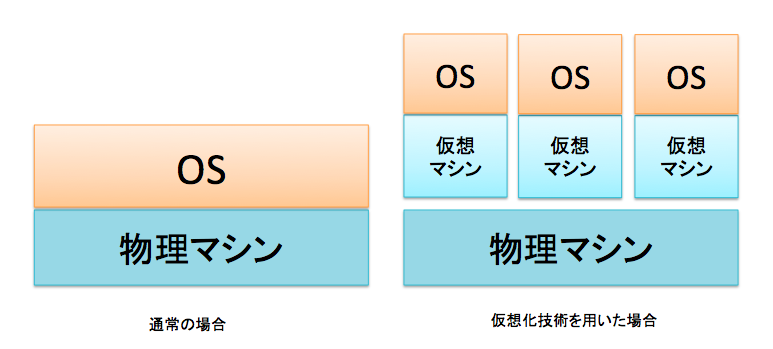
\includegraphics[width=8.0cm]{./img/virtual_tech.png}\caption{ サーバの仮想化}\label{virtual_tech}\end{center}\end{figure}

サーバの仮想化の利点は多々ある.その利点について説明する.
\begin{itemize}
\item リソースの効率的な利用\\
     サーバ仮想化を行わないと
マシン上では一つの OS しか起動できないため,一つの OS が全ての計算資源を占有する.
その唯一の OS が使用しない計算資源が存在する場合その計算資源を使用することはできない.
一方,サーバ仮想化を行うことで計算資源を複数の OS で効率的に分配し
有効に利用することができる.
\item システムの柔軟性\\
     サーバに与えられるのは仮想マシンのため,
多くの仮想マシンを一台の物理マシン上で稼働させることで多大数を一括で管理することができる.
またハードウェアのデバイスチェックなどの時間も省略できるので立ち上げの高速化や
Live Migration により仮想マシンを稼働させたまま他の物理マシンに移送することもでき,
物理マシンのメンテナンスも容易になる.
\item 省コスト・省電力\\
     物理サーバの運用台数を削減できるので電力の消費,設置スペースの削減が行える.
\item 障害性\\
     仮想マシンごとは完全に分離されているのでいずれかの仮想マシン上の OS がクラッシュしても
他のマシンには影響をあたえない.
\end{itemize}
このようにサーバ仮想化には様々な利点がある.

サーバの仮想化には様々な方法が存在する.
その方法は大きく二つに分類され,ホスト OS 型とハイパーバイザ型に大別される.

\subsubsection{ホスト OS 型}
\label{sec-2-1-3}
図\ref{host_vs_hyper} のように物理マシン上でひとつのホストとなる OS が稼働し,その OS 上で
仮想マシン・モニタを起動する方式.仮想マシン・モニタとは仮想マシンをゲスト OS に提供する
ソフトウェアの事を指す.ホスト OS 型は既存のマシン環境で,
他のアプリケーションを使用するようにインストールし,起動することが
できる.実際の例として Macintosh マシン上で
アプリケーションの VirtualBox\cite{virtualbox} などの仮想マシン・モニタを
用いて Windows を起動することができる.
仮想マシン・モニタに与えられる CPU 処理時間はホストマシンの OS の
アプリケーションへの CPU 割当スケジューリング依存になるので,ホスト OS で多くのアプリケーションを
起動している場合や多数のゲスト OS を起動している場合性能が低下する場合がある.
\subsubsection{ハイパーバイザ型}
\label{sec-2-1-4}
ホスト OS 型だと仮想マシンと物理マシンの間にはホスト OS と仮想マシン・モニタの二層が存在する.
一方ハイパーバイザ型では図\ref{host_vs_hyper} のように
物理マシンと仮想マシンの間にはハイパーバイザと呼ばれる
仮想マシン・マシンモニタのみが存在する.ハイパーバイザによってハードウェアは仮想化され
OS に提供される.ホスト OS が存在せずハイパーバイザが直に物理資源を利用するため
ハイパーバイザがゲスト OS へ与えられる CPU のスケジューリング行うことができる.
そうすることによりホスト OS 型と比べると,効率的にかつ安定的に CPU をゲスト OS に
割り当てることができる.vmware の vSphere\cite{vsphere},citrix の XenServer\cite{xenserver},
Microsoft の Hyper-V\cite{hyper-v}など
商用の仮想化ソフトウェアとしてハイパーバイザ型の商品も多数存在する.
オープンソースでの開発も行われていて,XenSever の元である Xen\cite{xen} や Linux カーネルに
マージされている KVM\cite{kvm} などがあげられる.
\begin{figure}[H]\begin{center}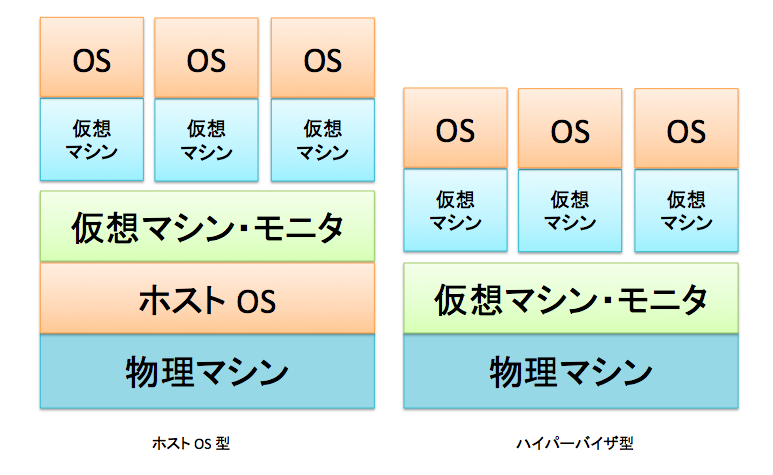
\includegraphics[width=8.0cm]{./img/host_vs_hyper.png}\caption{ ホスト OS 型とハイパーバイザ型}\label{host_vs_hyper}\end{center}\end{figure}

\subsubsection{完全仮想化と準仮想化}
\label{sec-2-1-5}
ハイパーバイザ型のサーバ仮想化には完全仮想化と準仮想化の二種類が存在する.
この二種類の違いについて図 \ref{full_para} を用いながら説明する.

\begin{itemize}
\item 準仮想化\\
      準仮想化では使用するゲスト OS に手を加える必要がある.
(図 \ref{full_para} の右)
準仮想化で提供される
仮想マシンはそのままの OS では使用できない API を提供する.
完全仮想化と比べて,仮想化に適した OS を使用することができるので
性能は上がるとされている.
OS の変更場所はカーネル部分となる.変更により OS が直接ハードウェアを操作する命令が
仮想マシンを通したハイパーコールなどに変更される.

準仮想化では仮想化によるオーバヘッドは削減できるものの,OS に手を加えなければならないため
変更に伴う管理コストがかかる.仮想マシン・モニタの更新ごとに OS を互換性を保ち移植しなくては
ならない.

研究の使用の面で考えると使い勝手が良い場合がある.
例えば,準仮想化された仮想マシンの OS は,自分が仮想化されていることを理解しているため
仮想マシン・モニタを操作するハイパーコールの使用が可能である.よって例えば
自分のメモリが実際に使用している物理アドレスを取得して自分で管理することもできる.
完全仮想化ではこのようなことはできない.

\item 完全仮想化\\
      完全完全仮想化では使用するゲスト OS に手を加えず使用できる.
(図 \ref{full_para} の左)
そのため,手を加えることのできない OS も起動することができる.
その例として Windows OS があげられる. Windows はソースコードが
開示されていないため,オープンソースの Linux などとは違い手を加える事ができない.

完全仮想化ではゲスト OS は自分が仮想化されていることを知らず,実際の物理マシンを
専有しているものと考える.そのため仮想化によるオーバヘッドが生じる場合がある.
しかし,準仮想化とは違い OS に手を加えないので管理コストが削減できる.

研究での使用の面で考えるとコードが簡潔になる場合がある.
完全仮想化ではゲスト OS の動きに関与しないため,
準仮想化では必要な処理が隠蔽され,必要な処理が減る場合がある.
そのため,コード量や考慮すべき点が減り,複雑なことをしないで済むので
バグが出にくくなる.
そのかわり,ゲスト OS でハイパーコールを実行できない.
\end{itemize}

\begin{figure}[H]\begin{center}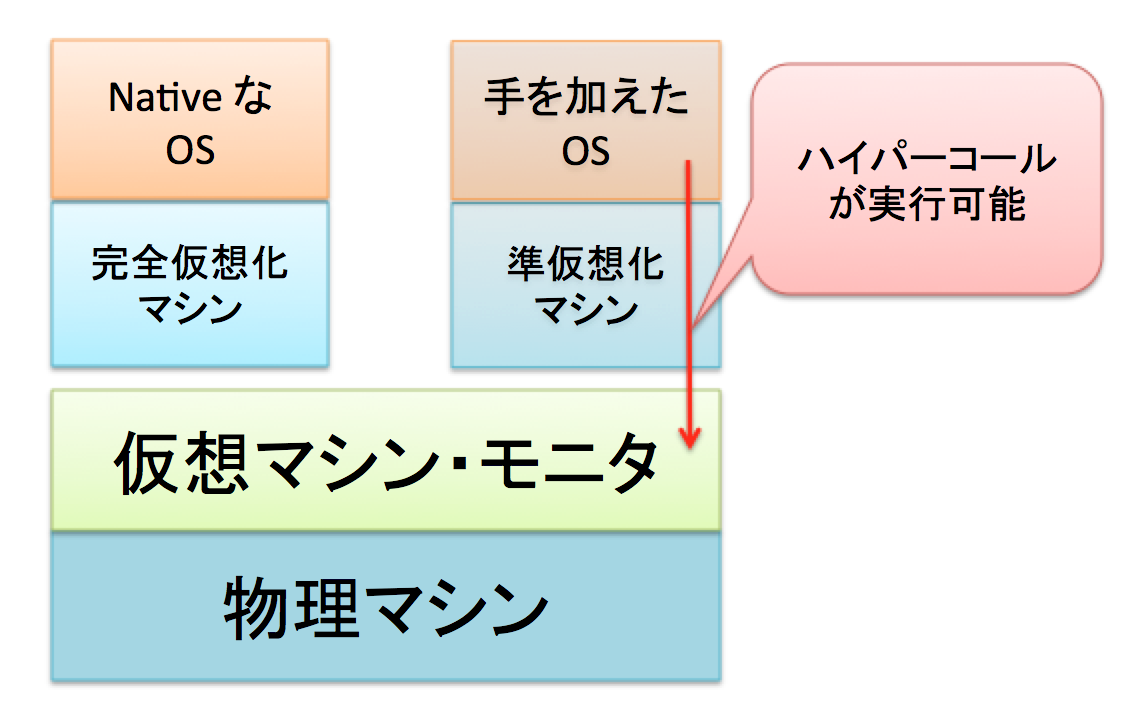
\includegraphics[width=8.0cm]{./img/full_para.png}\caption{ 完全仮想化と準仮想化}\label{full_para}\end{center}\end{figure}

\subsection{クラウドコンピューティングにおける仮想化技術の利用}
\label{sec-2-2}
\subsubsection{クラウドコンピューティングとは}
\label{sec-2-2-1}
クラウドコンピューティングとは,インターネットを介して,必要に応じた計算資源を
ユーザに提供するサービスである.ユーザは実際の物理マシンを意識せず計算資源を利用する
ことができる.

従来ユーザがシステムを構築しようとしたとき,物理マシンを用意し,
そのうえに基幹ソフトウェアをインストールし,必要な環境を用意することで
初めて利用を開始していた.また使用を開始した後も
物理マシンのメンテナンスから,ソフトウェアの環境の管理など様々な管理コストが掛かっていた.
一方クラウドコンピューティングでは必要な環境をユーザ登録などを済ませることで
すぐさま利用することができる.また利用するユーザは物理マシンのメンテナンスなどをサービス提供者に
任せることができる.
クラウドコンピューティングでは,下位層から上位層様々な層のサービスを提供する.
具体的には下位層では基幹ソフトウェアも何も用意していないようなマシンから
上位層であればソフトウェアのみのサービスなどである.
ユーザは自分の提供された計算資源より上位層の部分だけ管理すればよいので従来必要だった
管理コストを他に割り当てることができる.
例えばストレージのみをクラウドコンピューティングで利用する場合,
保存したファイルのバックアップ作業はサービス提供元が行ってくれるので
バックアップの為に RAID を構成するなどの管理作業からユーザは解放されることになる.

\subsubsection{PaaS とは}
\label{sec-2-2-2}
クラウドコンピューティングの一つのサービス体系で,アプリケーションが稼働するための
ハードウェアや OS などのプラットフォーム一式をインターネットを介して提供する
サービスである.

プラットフォームを提供されるユーザは開発,運用のためのハードウェアや OS ,開発環境,
ミドルウェアなどのプラットフォーム一式を自ら構築しなくてよい.
ハードウェアのメンテナンスや障害対応もしなくてよくなる.
またユーザは利用規模に応じたサービスを受けることができるので利用規模に応じた柔軟な計算資源の
利用をすることができる.

PaaS 提供者は,プラットフォーム一式を大規模なデータセンタなどに用意して,
顧客企業へネットワークを通じてプラットフォーム一式を提供する.
データセンタ内では複数の物理マシンサーバが用意され,プラットフォームの管理には
仮想化技術が利用されている.
各物理マシン上で仮想化技術により複数の仮想マシンが稼働しており,その各仮想マシン上に同様の構成の
プラットフォーム一式が構築される(図\ref{paas}).
ユーザにはその構築されたプラットフォームが提供される.
PaaS 提供者は各物理マシンの整備からミドルウェア,開発環境などの管理をすることになる.

具体的な一例として Microsoft の Azure\cite{azure} をあげてみる.
Azure のサービスは IaaS,PaaS,ストレージなど多岐にわたる.
そのうち, PaaS のサービスでは Azure Websites というサービスがある.
これは管理されたプラットフォームをユーザに提供し,ユーザはプラットフォーム上で
Python,Java,PHP,ASP.NET など様々な言語を使用しランタイムの Web アプリケーション
を使用することができる.
プラットフォームは Windows Serever に手を加えたものが使われており,
ミドルウェアなども含め多くの同じプログラムを起動している仮想マシンが複数個
データセンタの物理マシン上に存在している.

\subsection{Live Migration}
\label{sec-2-3}
\subsubsection{Live Migration とは}
\label{sec-2-3-1}
Live Migration とは,アプリケーションを稼働したまま仮想マシンを他の物理マシン上に移送する
技術である.
この機能により仮想マシン上で稼働しているサービスを止めることなく,仮想マシンを他の物理マシンへ
移送することができる.
Live Migration の機能は様々な仮想化ソフトに実装されている.
ホスト OS 型である,Virtualbox\cite{virtualbox}では「テレポート」という機能として,
ハイパーバイザ型では VMware の vSphere\cite{vsphere} では「VMotion」,
Citrix XenServer\cite{xenserver} では「XenMotion」,
Microsoft の Hyper-V\cite{hyper-v} やオープンソースの KVM\cite{kvm},
Xen\cite{xen}ではそのまま「Live Migration」という名前の機能として使われている.

\subsubsection{Live Migration の用途}
\label{sec-2-3-2}
Live Migration の用途について説明する.
まず複数の仮想マシンの負荷総量が物理マシンの処理能力を上回った
場合の利用についてあげる.
仮想化を導入する理由の一つにハードウェアの効率的利用があげられる.
高性能のハードウェアの計算資源を常に全て利用することは難しいので,
複数のサーバをその一台に集約することで計算資源を効率的に利用することができる.
しかしそのような使い方をすると一台の物理マシン上で稼働する各仮想マシンが
高負荷な処理を行ったとき,物理マシンの処理能力を複数の仮想マシンの負荷総量が上回って
しまうことがある.上回った場合,各仮想マシンへの CPU が割当が枯渇してしまい
各仮想マシン上で動いているサービスの性能が低下してしまう.
このような場合に図\ref{dispersion} のような Live Migration の使用が考えられる.
負荷総量の上昇を検知できた段階で一部の仮想マシンを他の物理マシンに移送すれば
負荷総量が物理マシンの処理能力を超さないで済む.
このとき仮想マシンのメモリ量が同じならば高負荷のマシンを移送するより
負荷の少ないマシンの方が短い移送時間で移送できる.
\begin{figure}[H]\begin{center}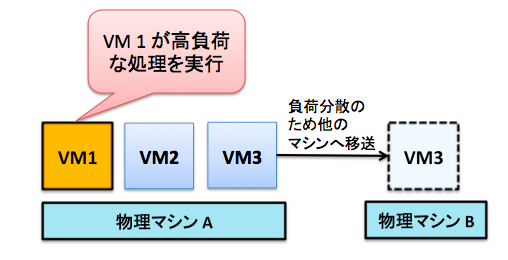
\includegraphics[width=8.0cm]{./img/dispersion.png}\caption{ 負荷分散}\label{dispersion}\end{center}\end{figure}

次にあげられるのが物理マシンのメンテナンスをする場合である.
ホストマシン上で稼働する仮想マシン・モニタはバグ修正,機能向上のために
定期的にパッチがリリースされる.そのため定期的にホストマシンを停止し,
仮想マシン・モニタを更新する.その他にもメモリの故障による
ハードウェアの交換時などにもホストマシンを一旦停止することになる.
ホストマシンを停止する場合,ホストマシン上の仮想マシンもシャットダウンされてしまう.
しかし仮想マシンでサービスを動かし続けている場合は,サービスを中断するわけにはいかない.
このような場合仮想マシンのサービスを停止することなく他のホストマシンに移送する
Live Migration が用いられる.
図\ref{maintenance} のようにLive Migration によってメンテナンスをしたい
ホストマシン上の全ての仮想マシンを
他のホストマシン上に待避させることができる.全ての仮想マシン待避後,
ホストマシンを停止してハードウェアのメンテナンスを行ったり,再起動を伴う
更新などを行うことができる.
\begin{figure}[H]\begin{center}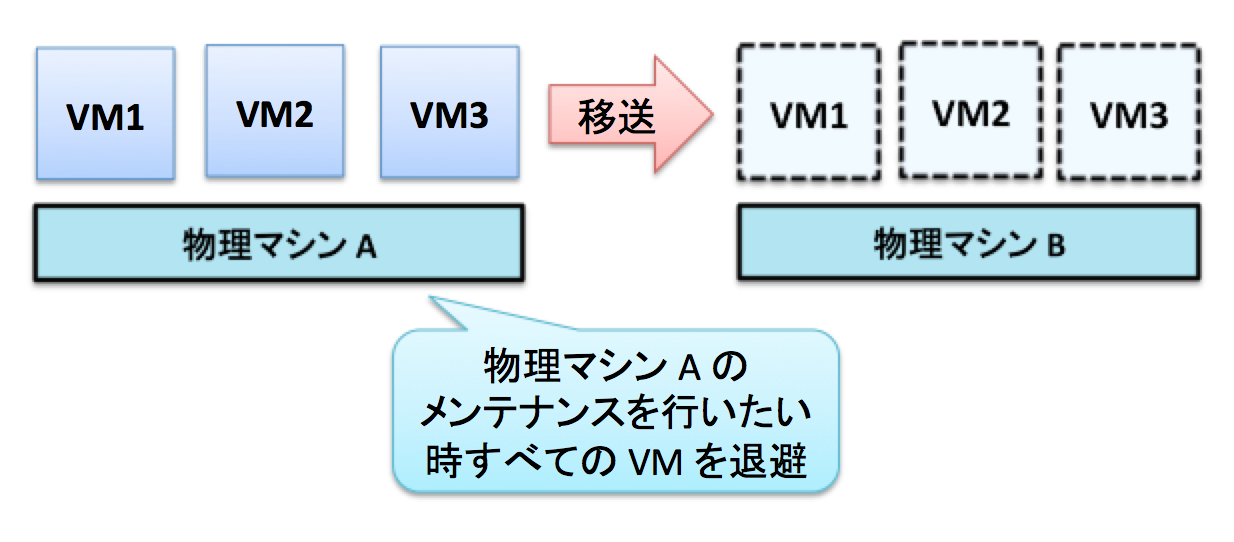
\includegraphics[width=8.0cm]{./img/maintenance.png}\caption{ 物理マシンのメンテナンス時 }\label{maintenance}\end{center}\end{figure}

\subsubsection{移送する対象と方法}
\label{sec-2-3-3}
Live Migration を行うにあたっての移送する対象と
その移送方法について説明する.
まず仮想マシンを移送するということは,大きく二つにわけて,
仮想マシンのディスクとメモリを移送するということになる.
この仮想マシンのディスクとメモリの移送方法は二つにわかれる.
一つはディスクとメモリ両方を移送先に移送する方法で,
もう一つは移送先とディスクを共有しておきメモリだけ移送する方法である.
\begin{itemize}
\item 両方とも移送先に移送する\\
      まず一つ目の移送方法は,仮想マシンのメモリとディスクを
どちらも移送する方法である.マシンの配置例は図\ref{arrangement1}
のようになる.
この場合移送先には VM2 の HDD と メモリを移送しなければならない.
まず VM2 の HDD を移送後,メモリを移送先に移送することで移送が完了する.
詳しい移送の仕組みについては後述する.
ディスクを共有する方法では共有ディスクを用意しなくてはいけないが
両方送れることで用意なしで Live Migration が可能になる.
しかし,ディスク送信をするため大きい容量を移送しなければならないのでネットワークを圧迫したり,
移送時間が長い.
他にも citrix の XenServer には Storage XenMotion \cite{Citrix:2011:SXL} として,
Microsoft の Hyper-V には Shared Nothing Live Migration という機能として実装されている.

\begin{figure}[H]\begin{center}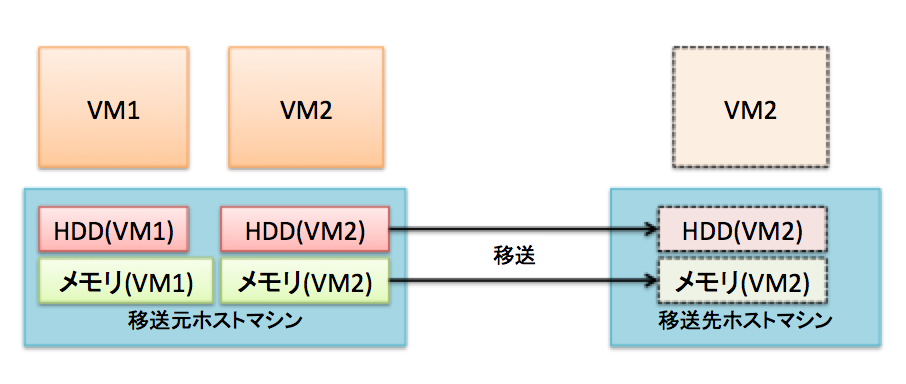
\includegraphics[width=10.0cm]{./img/arrangement1.png}\caption{ マシン配置例1}\label{arrangement1}\end{center}\end{figure}

\item ディスクを共有しメモリのみを移送する\\
      もう一つの方法は図\ref{arrangement2}の様にストレージを移送先と移送元で共有し,
メモリのみを移送先に移送する方法である.
移送の流れとしてはメモリを移送先に移送し,全て移送完了後,移送先の仮想マシンを稼働させる.
ストレージは共有ストレージを使用しているので送信しないで済む.
移送する対象がメモリだけなのでディスクとメモリ両方を移送する方法よりも
大きく移送時間を減らすことができる.
共有の方法には NAS(Network-attached storage)などがあげられる.
本論文での Live Migration はこの方法を指すものとする.
\begin{figure}[H]\begin{center}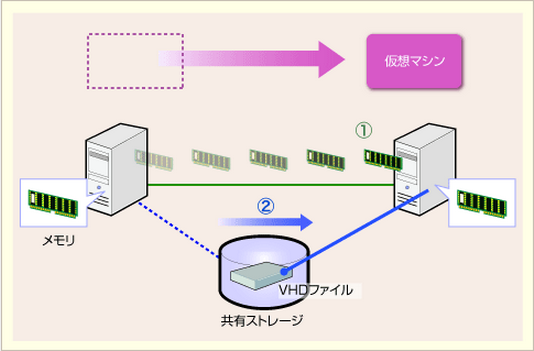
\includegraphics[width=8.0cm]{./img/arrangement2.png}\caption{ マシン配置例2この図は書き換える}\label{arrangement2}\end{center}\end{figure}
\end{itemize}

\subsubsection{移送の仕組み}
\label{sec-2-3-4}
\begin{itemize}
\item ストレージの移送\\
      本提案ではディスクを共有したメモリのみの移送をする Live Migration を使用するので,
ストレージの移送方法については vSphere の移送方法のみを参考として説明する.
図\ref{vmotion} \cite{Sreekanth:2012:VV5} のように
vSphere のディスク移送には並列して二つのプロセスが稼働する.
一つはストレージ全体を線形的に移送先にコピーする Bulk Copy プロセスと,
もう一つは IO をミラーリングするプロセスである.
IO ミラーリングのプロセスは OS の IO 操作を監視して,IO 操作を移送元ホストの
現在使用中のストレージと移送先ホストのコピー中のストレージに反映させる.
ふたつのプロセスはトランスポートのバッファリングを用いて非同期的に移送先に送信される.
何故バッファリングを行い非同期的に行うかというと,
同期的に行うと,ネットワークのレイテンシによっては IO がとても混雑してしまい,
VM の性能を下げてしまうことがあるからである.
Bulk Copy プロセスが全てのストレージを移送先にコピーすると,Bulk Copy プロセスは
終了し,IO ミラーリングプロセスのみが稼働し続けた状態でメモリの移送を開始する.
\begin{figure}[H]\begin{center}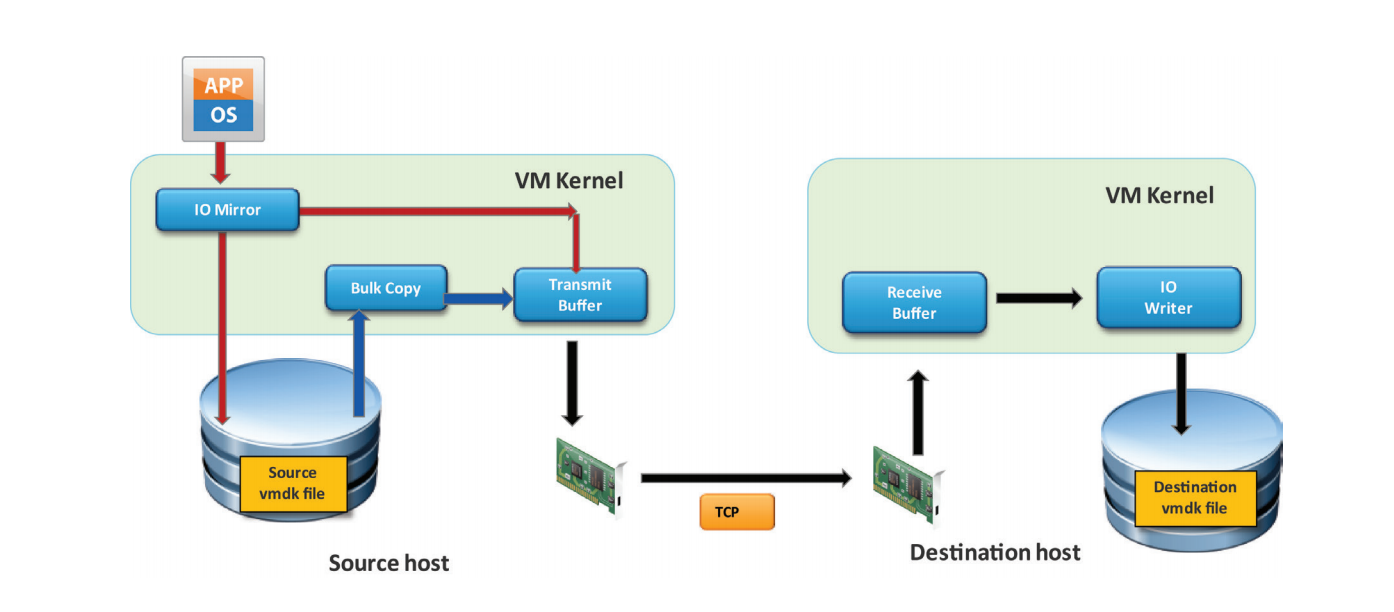
\includegraphics[width=12.0cm]{./img/vmotion.png}\caption{ ストレージ vMotion}\label{vmotion}\end{center}\end{figure}

\item メモリの移送\\
      メモリの移送は主に pre-copy \cite{Clark:2005:LMV} が使用されている.
vSphere\cite{vsphere} の vMotion(vSphere 特有の Live Migration の機能の名前)
\cite{Sreekanth:2012:VV5} 
や Hyper-V\cite{hyper-v} の Live Migration,
オープンソースの Xen などで実際に pre-copy が使用されている.
ここでは pre-copy について説明する.
pre-copy では六つのステージによって Live Migration を行う.
動作の流れを図\ref{pre-copy} \cite{Clark:2005:LMV} に示す.ステージ0では 移送したい VM を稼働
することができる程の計算資源を持った移送先ホストマシンを選択する.
ステージ1では移送先ホストに移送を開始することを通知する.また送信ができる程の計算資源が
あるかどうか確認する.ステージ2ではメモリを繰り返し送信する.このステージでは
まず全てのページを送信する.送信中には dirty にされるページ(稼働中の仮想マシンが更新したページ)を
記録しておく.後続のイテレートでは dirty にされたページを再送する.
ページの再送時にも dirty にされたページを記録し,後続のイテレートとそのページを再送する.
ステージ2の移送中に更新されたメモリを再送するという動作を,管理者が定めた一定の閾値に達するまで繰り返す.
閾値にはメモリの再送フェーズを行う回数の最大値や,再送するページの数の最小値などが用いられる.
例えば,再送するページの数の最小値を 4000 ページと決めておくと,
毎回の再送フェースで再送するページが 4000 ページを下回るとその場でステージ3にシフトする.
ステージ3では仮想マシンをサスペンドし,残りの dirty になったページや CPU レジスタや
プログラムカウンタなどを移送する.
この移送が終わった状態では,移送元ホストマシンと移送先ホストマシンに同様の仮想マシン
イメージがある状態になる.
ステージ5では移送先ホストが移送元ホストに移送が終了したことを通知する.
この通知により移送元ホストは整合性のとれたメモリの移送を完了したとして,移送元の
仮想マシンを廃棄する.よって仮想マシンのイメージは移送先のもののみになる.
ステージ6では移送した仮想マシンを再開する.
この時デバイスドライバの設定や,仮想マシンの IP アドレスの設定などを行う.
このよう流れで Live Migration は実現されている.

\begin{figure}[H]\begin{center}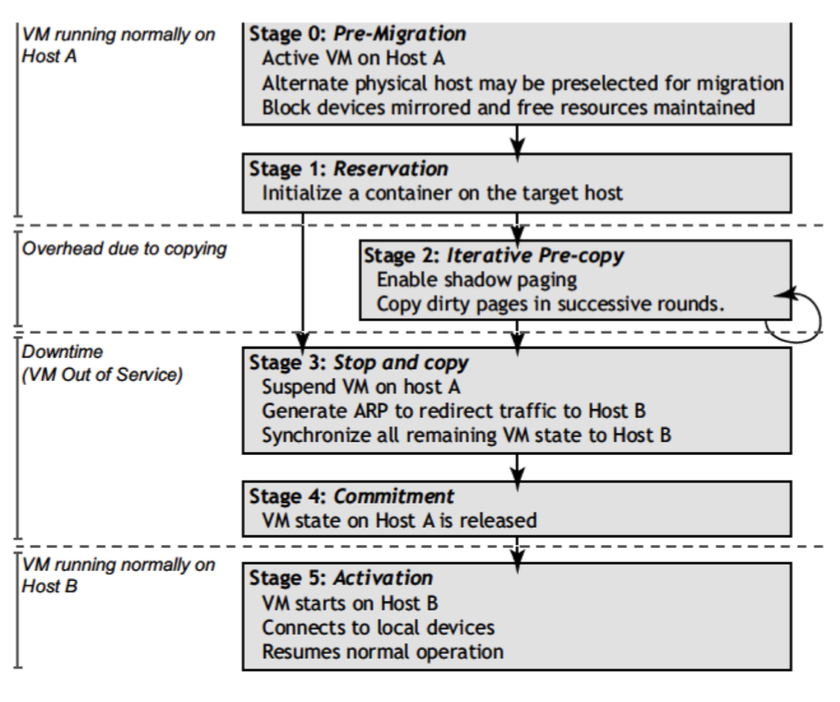
\includegraphics[width=10.0cm]{./img/pre-copy.png}\caption{ pre-copy の流れ}\label{pre-copy}\end{center}\end{figure}
\end{itemize}

\subsection{仮想マシン間のページ共有技術}
\label{sec-2-4}
仮想化技術により一つの物理マシンに複数台の仮想マシンが存在する場合,
各々の仮想マシンが同じ内容のメモリページを重複して持つ場合がある.
そのようなページを仮想マシン間で共有する方法を説明する.
\subsubsection{Transparent Page Sharing}
\label{sec-2-4-1}
\label{tps}
仮想マシン間で重複した内容のメモリページを共有する技術は
Disco\cite{Bugnion:1997:DRC}で 
{\it transparent page sharing}
として導入された.
同じ OS が起動していた場合,テキストデータ領域などが
共有できる場合がある.他にも同じアプリケーションを動かしているとき
そのアプリケーションのテキストデータ領域や,場合によっては使用する
データも共有できる場合がある.
そのような場合重複したメモリページに対して一つの物理ページを用意してやり,
どのメモリページもその一つの物理ページを参照する様にすればメモリの使用量を
減らすことができる.
重複排除したメモリページは読み込み専用に設定しておき,
書き込みを行った時に page fault が起こるようにしておく.
page fault が起きた場合,新しくページを作った上で変更した内容のページを作成する.
この手法は COW (Copy On Write) と呼ばれる.
上記の共有機能が実装される場合,仮想マシン・モニタに実装され,
ゲストマシン OS には共有されていることがわからないので
ゲスト OS には名前の通り透過的なメモリシェアとなっている.

\subsubsection{メモリ共有}
\label{sec-2-4-2}
\label{memory_share}
ここでは仮想マシンのメモリを効率的に共有する方法 \cite{Waldspurger:2002:MRM} を説明する.
メモリを共有するとき毎回 4kbyte のページ内容を全て比較していると計算量はかなり
多くなってしまう.また単にページ同士を総当たりで比べるとなるとページ数の自乗回の
比較が必要になってしまう.
そこで効率的な比較をする方法として
メモリ内容から計算されるハッシュ値によるハッシュテーブルの使用があげられる.\cite{Val:2003:AAC}
具体的には,図\ref{hashtable} のように
メモリの比較時にメモリの内容からハッシュ値を計算してハッシュテーブルから
同じハッシュ値をもつページを引く.もし同じハッシュ値を持つページが存在すれば
ページの内容を比較して,同じならば TPS (Transparent Page Sharing) で共有する.
もし同様のハッシュ値がなかった場合はハッシュテーブルに登録だけして終わる.

\begin{figure}[H]\begin{center}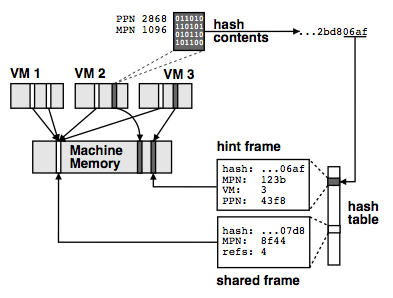
\includegraphics[width=8.0cm]{./img/hashtable.png}\caption{ ハッシュテーブルによるメモリ比較}\label{hashtable}\end{center}\end{figure}

このようにすることでページの内容が違う場合はハッシュ値の比較だけで済むため
比較の計算量が減る.またページの比較回数もページの自乗回かかっていたものが
ハッシュテーブルを利用して同じハッシュ値のみを検索し比較するので検索回数は大幅に減らすことができる.
検索が O(1) の理想的なハッシュテーブルを作成した場合は検索回数はページ数回で済むことになる.
しかし,仮想マシン・モニタがラージページに対応しているとページサイズは 4kB から
2 MB と 512 倍に跳ね上がるためページ共有の機会がとても少なくなる.
その場合共有をあまりしないのにハッシュ値を計算するために CPU を使用することになる.
またメモリの少しの変更で,2MB 分全ての内容を用いてハッシュ値を計算するため,
Microsoft では仮想マシンのページ共有は将来的に必要のないものになると考え
Hyper-V にはメモリ共有機能は実装されていない.
現在メモリ共有は ESX を内包する vSphere の TPS,オープンソースの KVM では
ivshmem(Inter-VM shared memory) という機能名で実装されている.
vSphere の TPS は機能の名前であって \ref{tps} の TPS とは本質的に意味が異なる.
本論文では特に指定がない場合 TPS という言葉は \ref{tps} の TPS を指すものとする.

\clearpage
\section{関連研究}
\label{sec-3}
\subsection{Post-copy}
\label{sec-3-1}
既存の仮想化マシン・モニタの Live Migration は主に pre-copy 方式が取られているが,
異なる方式も提案されている.それが,post-copy 方式\cite{Hines:2009:PBL}である.
pre-copy 方式が移送元で仮想マシンが稼働している中,移送先からメモリを送信する
のに対して,Post-copy 方式は一度仮想マシンの稼働に必要なデータのみを移送先に移送し,
移送先で稼働させ,必要になったページをその都度移送元から送信させるという方法をとる.
つまり大半のメモリを移送する時に,仮想マシンが稼働している場所が移送元か移送先かで異なる.
Post-copy ではページを送信するのは一回なので,
更新されたページを毎回再送する pre-copy 方式より送信量を減らし,
移送時間を短くすることができる.
Post-copy 方式の流れを図\ref{post-copy} に示す.
stage0 では Live Migration で移送できることのできる移送先のホストマシンを選択する.
stage1 の Stop and Copy では 仮想マシンを停止して,最低限の CPU のデータを送信する.
stage2 で pre-copy と同様に移送完了を確認し
stage3 で移送先の仮想マシンを再開する.
stage3 では再開した仮想マシンがアクセスしようとしたメモリが移送先になかったら
ネットワークを介して,移送元からメモリを取り寄せる.
取り寄せるとき pre-paging という方法を用いて,ページフォールトの回数を削減し,
仮想マシンの性能低下を抑える.
また Dynamic Self Ballooning という移送メモリ総量を削減する手法を用いて
メモリの送信量を削減し,移送時間を削減する.
全てのメモリを移送し終えたら,移送完了となる.
Downtime(仮想マシンがサービスを提供できない時間)
は stage1 と stage2 のみとなる.pre-copy と比べて
Downtime 中には CPU の最低限のデータしか送らないので Post-copy の方が
Downtime は短くなる.

\begin{figure}[H]\begin{center}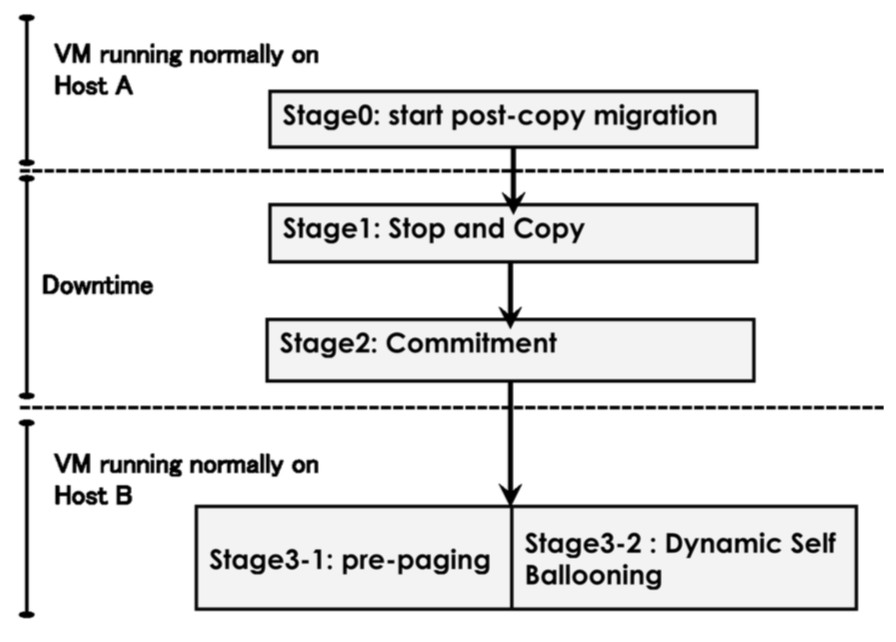
\includegraphics[width=10.0cm]{./img/post-copy.png}\caption{ Post-copy 方式の流れ}\label{post-copy}\end{center}\end{figure}

Post-copy では移送後の仮想マシンがメモリにアクセスを試みたとき,
もし存在しなかったら移送元からメモリを取り寄せる間,仮想マシンは処理待ちになる.
また移送直後の仮想マシンはメモリがほとんど移送できていないので,
fault が頻繁に発生し,仮想マシンの性能を妨げる場合がある.
そのため fault の回数を減らすため Pre-paging という方法が導入されている.
Pre-paging はメモリアクセスの局所性を利用した方法で,
移送先で必要になり取り寄せたメモリの周辺の番地を移送元が優先的に移送する方式である.
この手法によりネットワークを介したページフォルトの発生を,メモリ全体の 21 \% 以内
に抑えることができた.

またこの研究では Dynamic Self Ballooning という手法も導入している.
この手法はバルーニング \cite{Waldspurger:2002:MRM} の技術を応用して migrate するメモリ量を減らす手法である.
よってこの方式は Pre-copy 方式でも用いることができる.
バルーニングはメモリを管理する仮想マシン・モニタが仮想マシンに与えるメモリの量を動的に
変える技術である.バルーニングによりある仮想マシンのメモリが足りなくなった場合,
仮想マシン・モニタを通して,メモリが余剰となっている仮想マシンからメモリ領域をもらうことができる.
バルーニングの機能を実装するためにバルーニング技術には仮想マシンの使用していないメモリを
管理する機能が実装されている.この機能を使うことで,使用していないメモリを把握でき,
そのようなページを送信しないことで送信メモリ量を削減することができる.

この研究では PaaS 環境で仮想マシンの移送を行う場合,
移送先にも同様の内容のページがあるようなページを移送する.
そのようなページを送信しないようにすれば送信量を減らすことができる.

\subsection{移送メモリ量削減手法}
\label{sec-3-2}
Live Migration の転送メモリ量を削減して,移送時間を短くする研究\cite{Koto:2012:TUV}が行われている.
Live Migration は CPU の消費が大きく,ホストマシン上の移送する仮想マシン以外の
仮想マシンに影響を与える場合があることもこの研究では述べている.
図\ref{migrate-noise} では1台のホストマシン上で稼働する仮想マシン VM1 と VM2 の VM2 を
移送する場合,各仮想マシンのスループットが低下することを示している.
また,図\ref{migrate-noise-cpu}では,移送元に仮想マシン VM1 と VM2 があり,VM2 を移送した場合
CPU 使用率が移送管理用の仮想マシンに与えられることで,
他の仮想マシンへの CPU 使用率に影響が出ることを示している.
\begin{figure}[H]\begin{center}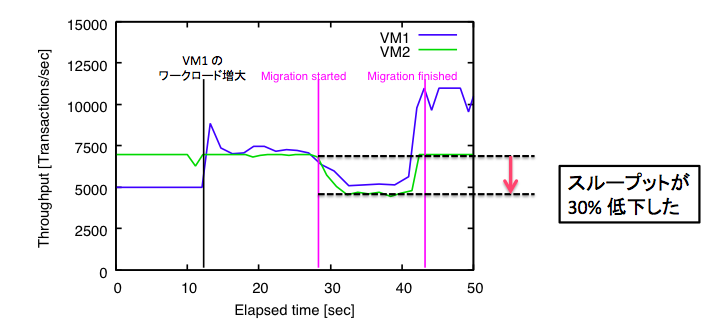
\includegraphics[width=12.0cm]{./img/migrate-noise.png}\caption{ 移送によるスループットへの影響}\label{migrate-noise}\end{center}\end{figure}
\begin{figure}[H]\begin{center}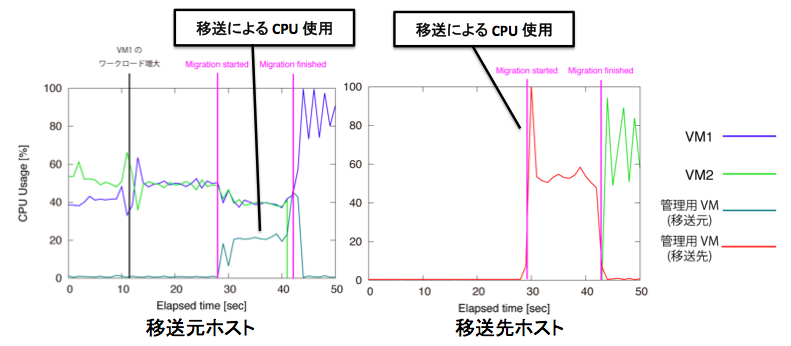
\includegraphics[width=12.0cm]{./img/migrate-noise-cpu.png}\caption{ 移送による CPU への影響}\label{migrate-noise-cpu}\end{center}\end{figure}

この研究ではソフトステートなメモリを非転送メモリの対象として,移送メモリ量を削減している.
ソフトステートなメモリとはファイルキャッシュなどのことである.
ファイルキャッシュなどは移送しなくても移送先で再構築が可能である.
この手法により,この研究では既存手法より最大で 83.9\% の
ページの転送を削減することができた.

この研究に関しても PaaS 環境にて仮想マシンの移送を行う場合,
移送先にも同様の内容のページがあるようなページを移送する.
そのようなページを送信しないようにすれば送信量を減らすことができる.

\subsection{メモリ共有手法}
\label{sec-3-3}
\ref{memory_share} で述べたメモリ共有手法のように,
仮想マシン間でメモリを共有する方法 \cite{Waldspurger:2002:MRM} が提案されている.
メモリの共有手法に関しては \ref{memory_share} で述べた通りである.
この研究では実際に仮想マシン間でどのくらいのメモリを共有できるかを実験している.
その実験の結果を2つ示す.
1つ目の実験が OS が Red Hat Linux7.2,メモリが 40 MB の同じ設定の仮想マシン
を1台から10台まで起動し,並列して起動する仮想マシンには SPEC95 ベンチマークを
30分動かし,共有できるメモリの量を測定したものである.
結果を図 \ref{MRM_exp1} に示す.
上の図は仮想マシンの起動数に応じた,仮想マシンのトータルのメモリ量,共有されている
ページ数,共有で回収できたページの量,0ページの数を示してる.
0ページはページの内容が0で埋められた OS によって初期化されたままのページである.
上の図では仮想マシンが1台から2台になる時に仮想マシン間で共有できているページ数が期待するとおりに
増えていることが見て取れる.
これらの共有できているページは重複した内容のメモリやテキスト領域などの read-only な
ページである.
下の方の図は全体のメモリの量と比べた共有できているページの割合,回収できたページの割合,
実際に COW にして存在する共有メモリを参照した時に参照される物理ページの割合である.
この結果ではシェアされたページの割合があまり変動せず,共有メモリの参照物理ページの割合が
減っていくのがわかる.
仮想マシンが増えても共有できるのはワークロードで重複したページや,テキスト領域などの
read-only のページなので,シェアする内容は変わらないため実際に参照するための物理ページ
を1回用意してしまえばそれを再利用できるため,参照物理ページの
割合は減っていくが共有は同じ量だけ行えているので共有できたページの割合は変動しない.
このことから同じ OS で同じワークロードの仮想マシン間では 67\% 近くのページを共有することが
できることがわかった.

\begin{figure}[H]\begin{center}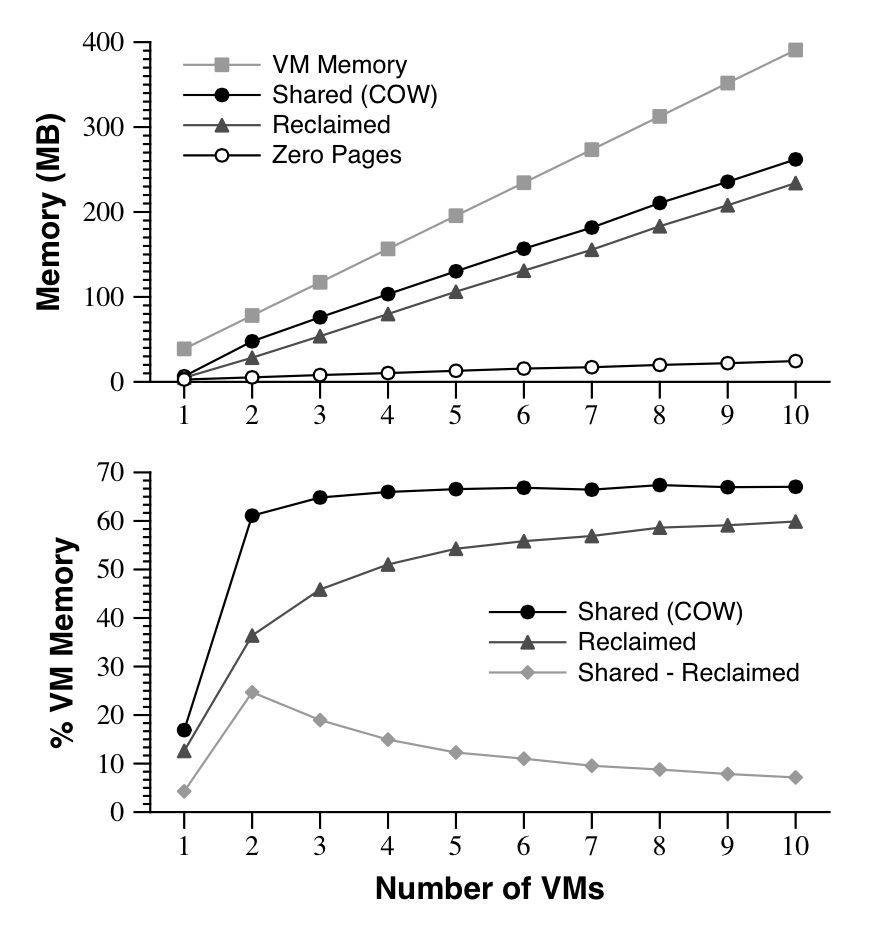
\includegraphics[width=8.0cm]{./img/MRM_exp1.png}\caption{ メモリ共有実験1}\label{MRM_exp1}\end{center}\end{figure}

二つ目の実験は共通の OS で似たようなアプリケーションを動かした仮想マシン間での
共有である.
これは real-world サーバの使用ワークロードがこのような使い方をするからである.
実験結果を表 \ref{MRM_exp2} に示す.
実験 A では10個の Windows NT 4.0 を稼働して,それぞれ
データベースやウェブなどのサーバとして用いる.このワークロードは Fortune 50 社の IT 部門
のものである.
データベースには Oracle, SQL Serever, ウェブには IIS, Webphere などを用いている.
結果 30 \% 強のメモリを共有により回収することができた.
実験 B ではある非営利団体のインターネットサーバで使用されている9個の Linux 仮想マシンを対象とした.
各仮想マシンのメモリサイズは 64 MB から 768 MB でメール,ウェブ,その他のサーバとして使用している.
メールでは Majordomo, Postfix, POP/IMAP, MailArmor,ウェブでは Apache などを用いている.
この実験では18.7 \% のメモリを回収することができた.回収できた 345MB のうち 70MB は0ページに
よるものだった.
実験Cは VMware の IT 部門のワークロードでウェブプロキシ,メール,VMware の
従業員のためのリモートアクセスサービスの為に使われている 5 個の Linux 仮想マシンを対象にしたものである.
ウェブプロキシには Squid,メールには Postfix, RAV,リモートアクセスには ssh を用いている.
各仮想マシンのメモリサイズは 32MB から 512MB である.
この場合は 7\% の回収をし,120MB のうちの 25MB が0ページによるものであった.

これらの実験から共有できるメモリの量はワークロードに依存することがわかる.
実験1のように同じ OS で同じワークロードであるようなマシンでは
共有率は 60\% に到達することがわかった.しかしワークロードによっては
同様の OS であっても 7\% しか共有できない場合があることもわかった.
本研究の PaaS 環境では,同様の OS 上で PaaS を管理するためのアプリケーションなど
様々な同様のアプリケーションを稼働することが想定される.
提供される PaaS 上ではユーザ個人のワークロードを動かすので,
共有が確実に見込まれるのは OS のテキスト領域や PaaS 管理のためのアプリケーションの
共有可能なメモリである.この場合だと完全にワークロードが等しくなるわけではないが,
いくつかの同様なワークロードは稼働していることになるので共有率はある程度は望めることが
この研究からも想定できる.

この研究ではメモリの共有後共有情報を利用はしていない.
このメモリ共有情報を用いれば,PaaS 環境で移送する仮想マシンが移送先で
再利用可能なページを効率的に見つけることができる.

\begin{table}[H]
\caption{メモリ共有実験2} \label{MRM_exp2}
\begin{center}
\begin{tabular}{|l|l|l|l|l|l|l|}
\hline
&               &  Total  &  \multicolumn{2}{|l|}{Shared}  &  \multicolumn{2}{|l|}{Reclaimed}  \\
\hline
&  Guest Types  &  MB     &  MB     &  \%                  &  MB     &  \%  \\
\hline
A  &  10 WinNT      & 2048    &  880    &  42.9                &  673    &  32.9    \\
\hline
B  &  9 Linux       & 1846    & 539     &  29.2                &  345    &  18.7    \\
\hline
C  &  5 Linux       & 1658    & 165     &  10.0                &  120    &   7.2   \\
\hline
\end{tabular}
\end{center}
\end{table}

\subsection{まとめ}
\label{sec-3-4}
Live Migration のために CPU やネットワークを消費し,
移送する以外のホストマシン上の仮想マシンにも影響を与える場合があることがわかった.
それに対して,メモリの転送量を少なくし,Live Migration の移送時間を短縮し,
CPU やネットワークの使用量を少なくする研究がなされている.
PaaS 環境における,移送する仮想マシンの移送先でも再利用可能なページを
転送しないことによるメモリ削減手法は提案されていない.
また仮想マシン間の同様のメモリを共有する手法も提案されていて,実際に同じ OS で
ワークロードによっては 67\% の共有率がでることもある.
メモリの共有により仮想マシン間でどのページが等しい内容を持つかといったような
メモリの共有情報を利用してはいない.

本研究ではメモリの共有情報を利用することで PaaS 環境における,
移送する仮想マシンが移送先でも再利用可能なページを効率的に探し,
それらのページを移送しないことでメモリの転送量を少なくする.

\clearpage

\section{提案手法}
\label{sec-4}
\subsection{概要}
\label{sec-4-1}
図\ref{paas} のように PaaS 環境においては同じ OS やミドルウェアを動かしている
仮想マシンが多く存在する.
よって,移送元の仮想マシンと同じ内容のメモリが移送先にも存在する場合がある.
本提案では PaaS 環境においてそのようなメモリを Live Migration 時に
移送先でメモリを共有することで移送せず,メモリの送信量を少なくする 
{\it SharingMigration}
を導入する.
メモリ送信量を削減することで CPU 消費や,ネットワークの消費を抑え
移送時間も減らす.

\subsection{SharingMigration}
\label{sec-4-2}
本提案では PaaS 環境を前提とした,移送先で共有可能なメモリページを送らないことによる
メモリ転送量を削減した Live Migration を 
{\it SharingMigration}
として導入する.
SharingMigration では4つのステージがあり,
その流れを図\ref{sharing_migration} に示す.
stage0 では移送元ホストマシン上で共有可能なメモリが仮想マシン間で共有されている
ゲスト OS が稼働している.
stage1 で移送する仮想マシンを決定し,移送することができる状況の移送先ホストマシンを
選択した後,\ref{non_migration_pages} の決定方法により非転送ページを決定する.
非転送ページは移送先で共有できるページなので,移送先では非転送ページに決まったページは
移送仮想マシン用に用意したメモリの参照を共有可能なメモリの物理ページに割り当てることで
共有する.
stage2 では非転送ページに決まったページ以外のページを pre-copy 方式で Live Migration する.
この Live Migration は非転送ページを移送しない以外は既存手法と同じである.
よって stage1 で移送先で共有可能なため非転送ページとなっていたページがもし更新されたとしても
そのページは再送される.

\begin{figure}[H]\begin{center}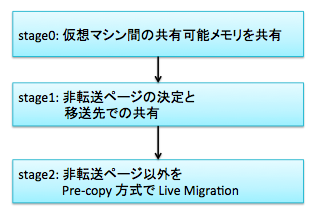
\includegraphics[width=8.0cm]{./img/sharing_migration.png}\caption{ SharingMigration の流れ}\label{sharing_migration}\end{center}\end{figure}

\subsection{非転送可能なページ}
\label{sec-4-3}
\label{non_migration_pages}
非転送ページの効率的な検索の方法について説明する.
非転送可能なページを検索する時,移送元と移送先で同じ内容のメモリ
がないかを総比較すると比較回数はページ数の自乗になってしまう.
また比較する時に,比較のためにページの内容を全て送るのでは
結局ページを全て送る事になってしまう.
そこで\ref{memory_share}でも使われている compare-by-hash \cite{Val:2003:AAC}
の手法を用いる.
メモリの内容比較をハッシュテーブルを用いて, \ref{memory_share} と同様比較回数を大幅に
削減することができる.
また移送先と移送元では比較のためにハッシュ値のみしか送らないため
全てのページの内容を送らなくてもページを比較することができる.
\ref{memory_share} ではハッシュ値の比較後,もしハッシュ値が同じでも,
メモリの内容が異なるものから同じハッシュ値が生成される場合を考慮して
メモリの内容を全て比較して確認をしている.
本提案ではメモリの内容比較のために移送先に全てのメモリを移送するのでは
メモリ転送量削減を行えないため,比較ではハッシュ値比較のみを行う.
もし比較後,移送したいページが移送先にもあり移送先で共有可能な非転送可能なページであった場合,
ハッシュ値計算に SHA-1 を用いると,ハッシュ値は 160 bit なので
ページの4096 byte と比較すると 99.5\% のネットワーク消費を抑えることができる.

ハッシュ値のみの比較は異なる内容のメモリから同様のハッシュ値が計算されてしまい,
異なる内容のメモリ同士を同様の内容と判断する場合がある.
しかしハッシュ値の衝突の確率は SHA-1(160bit)で 48 nines("0." の後に続く "9" の数が 48 個という意味)
で,TCP のブロック転送のネットワークで起るエラー確率の 8(または 9) nines より小さい.
TCP を使用する際は,ハッシュ値の衝突より大きいエラー確率のもと毎回
TCP を使用していることになる\cite{Val:2005:GUC}.
そのことを考えれば,ハッシュ値の衝突確率は取るに足らないものである.

さらに PaaS 環境を対象にすることでメモリの比較回数を少なくする.
PaaS 環境では図 \ref{paas} の様に複数の物理マシンの各マシン上で
同じ OS を動かした仮想マシンが稼働しているので OS のテキスト領域など同じ内容のメモリを持つ
仮想マシンが多く存在する.
本提案では PaaS 環境特有の同じ OS,ミドルウェアなどで構築された
各仮想マシンが,共通して持つメモリページを非転送ページの主な対象とすることで
更新が多いメモリなどの共有が行える場合が少ないメモリの比較を省略しメモリの比較回数を減らす.
具体的には,移送元の仮想マシン間で共有できているメモリページは
PaaS 環境特有の各仮想マシンが共通して持つメモリページを含むので,
移送元で共有済みのメモリページを非転送ページの候補とする.
非転送ページの候補のページのみ移送先のページと比較することで同様のページが
存在するかの確認比較回数を減らす事が出来る.

このように compare-by-hash や PaaS 環境の特徴を利用した方法で
移送元と移送先の共有可能で移送せずに済むページを効率的に比較して見つけることができる.


\subsection{非転送ページと送信量}
\label{sec-4-4}
Live Migration は移送中も仮想マシンが稼働しているためメモリを移送しても
更新されてしまい再送する必要がある.
よって移送時間が長い程更新されるページ数が増えて再送するページ量が増えるので,移送量が増えてしまう.
逆に移送時間が短くなる場合は,再送される量が減る.
ここで重要なのが,再送される量が減ることでまた移送時間が短くなり,さらに再送される量が少なくなること
である.つまり Live Migration において移送時間を削減すると
その効果は指数関数的に減少する.


\clearpage
\section{実装}
\label{sec-5}
\subsection{XEN}
\label{sec-5-1}
SharingMigration を実装する仮想マシン・モニタにはオープンソースでハイパーバイザ型の XEN を用いる.
XEN のアーキテクチャを図\ref{xen_structure}に示す.
XEN はハイパーバイザ型だが,ドメイン0とよばれる特別なドメインが存在する.
ドメイン0は管理用ドメインのホスト OS として存在してゲスト OS のドメイン U とは区別される.
XEN はドメイン0のホスト OS のデバイスドライバなどを利用することで,
ハードウェアの管理のコストを軽減している.そのためドメインU がデバイスの操作を行うと
その動作は XEN を一旦通した後,ドメイン0のデバイスドライバを用いて物理マシンへと反映される.
見方によってはホスト OS 型のように間違えられるかもしれないが,ドメイン0も実装上は
XEN 上で仮想化された仮想マシンの一つとして扱われており,
ホスト OS 上で仮想マシン・モニタが稼働しているのとは異なるため
XEN はハイパーバイザ型に分類される.
しかし,ドメイン0が XEN にとって特別なドメインであることは変わらず,
XEN などの操作をする場合ドメイン0からしか実行できない関数があったり,
Live Migration の移送の対象にすることができないなどドメイン U とは大きな違いを持つ.

ドメイン U の管理などの XEN の操作はドメイン0上から行う.
XEN の操作は主にハイパーコールとよばれる関数を用いて行う.
ハイパーコールとは仮想化を行っていない OS でアプリケーションが用いるシステムコールと似たものである.
システムコールはアプリケーションが OS の機能を呼び出すために使用する機構のことであるように
ハイパーコールはホスト OS が XEN の機能を呼び出すための機構である.
ハイパーコールのみでは実際に管理に使用するとき,使い勝手が悪いためハイパーコールを
ユーザが使い易いようにするため XEN にはツールが二種類存在する.
ひとつは xend という管理のためのデーモンプログラムをドメイン0のホスト OS 上で
起動し,xend を通してホスト OS がハイパーコールを実行するタイプの XM ツールである.
XM は python で書かれている.
もうひとつは xend などを通さずにハイパーコールをホスト OS が呼び出す XL ツールである.
XL ツールは C 言語で書かれている.
どちらのツールでもライブマイグレーションは可能である.
今回は研究室の先輩が XM を用いていることもあり XM ツール
を用いる.

\begin{figure}[H]\begin{center}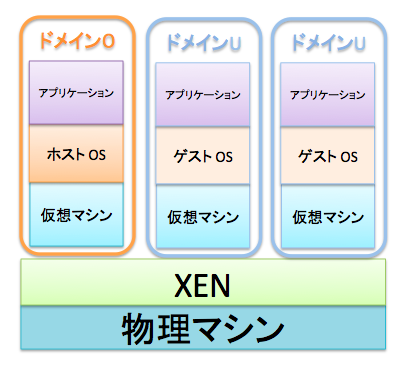
\includegraphics[width=8.0cm]{./img/xen_structure.png}\caption{ XEN の構造}\label{xen_structure}\end{center}\end{figure}

XEN のメモリの管理について説明をする.
XEN は図 \ref{fn} のように実際の物理マシンのメモリを仮想化し,仮想マシンの物理メモリとして
ゲスト OS にメモリを提供している.
XEN がメモリを管理するために,XEN ではメモリのアドレスをフレームナンバとして扱う.
ゲスト OS が占有していると考えている物理メモリアドレスは
XEN によって仮想化された仮想マシンのメモリの物理アドレスであるため
実際の XEN が管理しているメモリの物理アドレスと異なる.
そのため XEN はフレームナンバの種類を分けて管理する.
完全仮想化の場合は
実際の物理メモリの物理アドレスを扱う場合は MFN (Machine Frame Number)で扱い,
ゲスト OS から見た仮想マシンの物理アドレスを PFN (Physical frame number) として扱う.

\begin{figure}[H]\begin{center}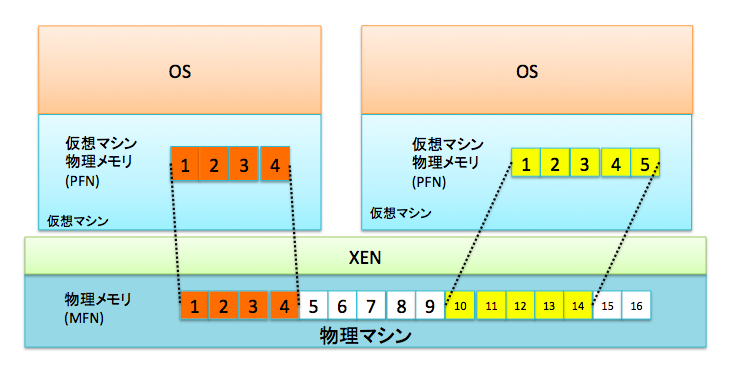
\includegraphics[width=12.0cm]{./img/fn.png}\caption{ XEN のメモリ管理}\label{fn}\end{center}\end{figure}

\subsection{メモリ共有モジュール}
\label{sec-5-2}
\ref{memory_share} で述べた様に
 現在仮想マシンのメモリ共有は ESX,オープンソースの KVM で実装されている.
 今回使う XEN には TPS の機能は実装されていたものの,ESX で使用されるような
 本格的なメモリ共有機能は実装されていなかったため実装を行った.
 ESX ではシェアリングを行うのにページの内容からのハッシュ値の計算,
 ハッシュ値が一致した場合ページ内容の比較,内容も一致した場合は
 シェアリングをする.よってシェアするための各処理に CPU 割当を必要とする.
 そのため ESX では一括ではメモリの共有をせず
 少しずつ時間をかけて共有をする仕組みを作っている.
 よって ESX では使用を続けていればバックグラウンドで少しずつ共有メモリが増えてゆく.
 そして,十分な時間がたつと,OS のテキスト領域などの固定されたデータは全て共有され
 ,いくらかのワークロードに依存した同じ内容のメモリも共有される.

本提案では仮想マシンは十分な時間稼働していたものを想定するため,
シェアできるような固定的なデータは全てシェアされているという状況を作り出せば良いため,
メモリの比較などは一括で行えるものを実装した.
このような実装をすると,シェアのために使用される CPU 処理が
仮想マシンの処理能力に影響を与える場合が考えられるが本実験では考慮しなくてよい.

具体的な実装デザインは ESX \cite{Waldspurger:2002:MRM}と同様である.
図 \ref{sharing_module} のように
仮想マシン・モニタの XEN 上にメモリの内容管理用のハッシュテーブルを配置した.
自作ハイパーコールの hash\_reg 関数がドメイン0で呼び出されると
引数で指定された仮想マシンのメモリ内容からハッシュ値を計算して,XEN 上の
ハッシュテーブルに登録される.ハッシュテーブルはドメイン事に個別のハッシュテーブルを
作成し,ハッシュ値と共に PFN を登録する.
またハッシュテーブルへの登録時にハッシュ値が衝突する場合がある.
この場合はメモリの内容を確認して,もし内容が同じだった場合 TPS により共有する.
この共有は仮想マシン間の共有ではなく,仮想マシン一台上での同様のメモリの共有となる.
もし起動後間もない時にこの関数を呼ぶと,zero page がシェアされ,大半のページが
解放されることになる.

\begin{figure}[H]\begin{center}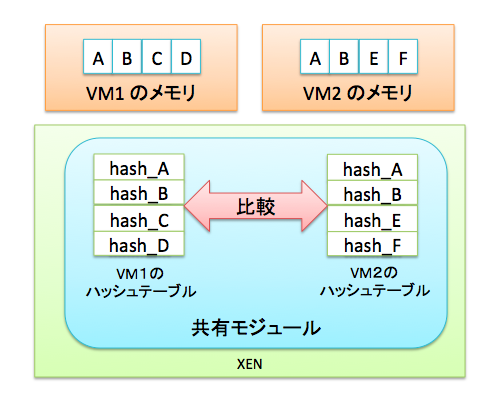
\includegraphics[width=8.0cm]{./img/sharing_module.png}\caption{ 共有モジュール}\label{sharing_module}\end{center}\end{figure}

hash\_reg によって仮想マシンごとのメモリ内容から計算したハッシュテーブルを作成することができた.
次に,hash\_share 関数で作成したハッシュテーブルを元に,ハッシュ値を比較していく.
比較方法は単純で,ソースとなるハッシュテーブルから全走査によって,一つずつハッシュ値を取り出し
もう片方のハッシュテーブルからハッシュ値を引き,一致したら内容を比較し,内容も一致したら
TPS で共有するという仕組みである.こうして指定した仮想マシン間の共有メモリをシェアすることができる.

この機能は一度使って終了する分には,ハッシュテーブルを作り共有して終了することができるのだが
実験で何回にもわたりハッシュテーブルを作る場合,ハッシュテーブルなどの管理もしなくてはいけない.
ハッシュテーブルは仮想マシン・モニタ上にあるため,ハッシュテーブルを作成して使用しなくなった後も
ハッシュテーブルを残したままだとメモリが枯渇してしまう.枯渇すると次のハッシュテーブルが作れないなどの
問題が起きたり,他の XEN の機能でメモリが足りない事によるエラーが発生する場合がある.
そこで renew\_hash ハイパーコールを作成した.
この関数は実験で使用した仮想マシンがもう存在しない場合,その仮想マシンが使用していたハッシュテーブルや
本実験のために用意したメモリを管理するための情報などを全て解放する関数である.
ハッシュテーブルは list.h マクロの 双方向リストを使用して実装しているのだが,最初 list.h の
双方向リストの要素を全走査するマクロ list\_for\_each の使い方を誤ったため for 文が回らず
最初の要素のみしか解放できていなかった.そのメモリリークにより数回 Live Migration をすると
メモリ不足により Live Migration が失敗するなどのエラーが起きた.
このときデバックの役に立ったのが XEN 上でメモリを確保する時の関数 xmalloc のエラーメッセージであった.
このようにシステムコールなどのエラーメッセージが重要であることがわかった.
そもそも仮想マシンをシャットダウンするタイミングでハッシュテーブルなどを消去する関数を呼び出すように
設定するのが通常考えられる設計だが,作成当時はシャットダウン周りのコードを理解していなかったため
このような方法となっている.

\subsection{SharingMigration の実装}
\label{sec-5-3}
\subsubsection{SharingMigration の実装面の流れ}
\label{sec-5-3-1}
SharingMigration 実装面での流れを移送先,移送元で区別して
図 \ref{sharing_migration_imp} に示す.
各ステージについて説明する.

\begin{figure}[H]\begin{center}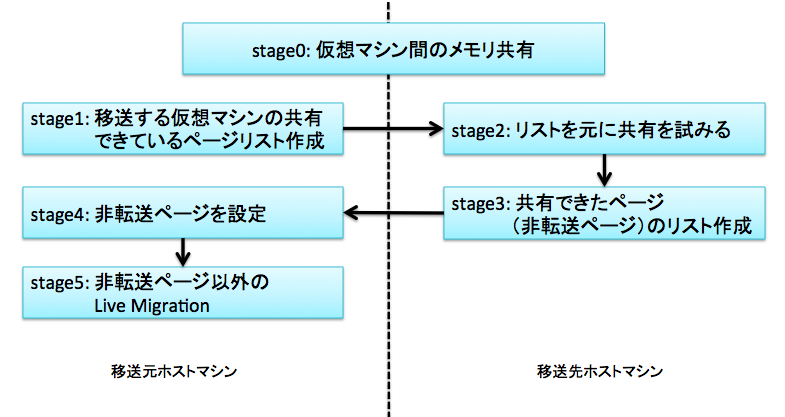
\includegraphics[width=12.0cm]{./img/sharing_migration_imp.png}\caption{ 実装面での SharingMigration の流れ}\label{sharing_migration_imp}\end{center}\end{figure}
\subsubsection{STAGE0,STAGE1}
\label{sec-5-3-2}
stage0 では移送元,移送先どちらも PaaS 環境の元で各仮想マシン間の共有できるメモリを共有する.

stage1 では非転送ページの候補のハッシュ値とそれに対応する移送仮想マシンの
PFN のセットをリストにまとめ,移送先に送る.
\ref{non_migration_pages} で述べた様に,非転送ページの候補は
移送元の仮想マシン間で共有しているページとする.
今回の実装では1台の仮想マシン上で共有できたページも候補に含んでいる.
この機能は hash\_lookup ハイパーコールで実装されており,ドメイン0で
呼び出すと,その時点で共有しているページのハッシュ値と PFN のセットのリスト,
セット数を取得することができる.
hash\_lookup の XEN 上で動くコードでは,移送する仮想マシンのメモリ共有モジュールで
作成されたハッシュテーブルを参照し,共有されている PFN を検索する.
ハッシュテーブルの一つのエントリにはハッシュ値が一つとメモリの内容を計算すると
そのハッシュ値が求まる PFN のセットが,2つもしくは複数リストで管理されている.
実際には共有できていたとしても(完全仮想化では関係ないが)ページテープルで使用されるページや
XEN\_DOMCTL\_PFINFO\_BROKEN などの属性を持つ特別な処理が必要なページは
非転送ページの候補から外す.
\subsubsection{STAGE2,STAGE3}
\label{sec-5-3-3}
stage2 では移送先から受け取った非転送ページ候補のリストを元に共有を試みる.
具体的には受け取ったハッシュ値のリストを移送先のホストマシンの仮想マシンのハッシュテーブルで
引いて,ハッシュ値が一致したら共有する.\ref{non_migration_pages} でも述べたように
ここではハッシュ値のみの比較でページ内容が一致するか判断する.
この時点では移送する仮想マシン用にアロックされている何も書き込まれていない空のページが
用意されており,共有が出来る場合はアロックした PFN に対応する MFN を解放して,
PFN の参照先 MFN を共有元の MFN のアドレスに書き換えてやることで共有ができる.

このステージで要となるのは移送先でハッシュ値が一致した場合,共有する前に
そのページのハッシュ値を再計算しない点である.
ハッシュ値を計算するのは hash\_reg 関数であることを述べたが,
図 \ref{non-renewal} のようにハッシュ値を計算した後にメモリの内容が更新される場合がある.
このとき登録された PFN に対するハッシュ値が正しくなくなってしまう.
しかし毎回更新事にハッシュ値を計算すると,CPU をとても消費していしまう.
また更新が激しいような共有できないメモリもあるので,更新ごとにメモリのハッシュ値
を再計算するのは現実的でない.
よってハッシュ値の計算後はメモリが更新されても,ハッシュ値は更新しない実装とした.
そのため移送先でハッシュ値が一致しても,そのハッシュ値が現在のメモリの内容に一致しているか
判別できない.
そこで最初はハッシュ値が一致した場合は移送元でそのメモリページの内容からハッシュ値を再計算して
メモリの内容とハッシュ値が一致することを確認していた.
しかしこの方法だとハッシュ値の再計算がオーバヘッドとなり移送時間が大きくなるため
非転送ページが少ないと移送時間が既存手法より大きくなってしまった.
SharingMigration で対象とするのは PaaS 環境特有の各仮想マシンが共有して持つページなので
頻繁に更新されるようなページは対象としないことから,
ハッシュ値が一致した場合でもハッシュ値計算後から1度でも更新されていたらその一致は考慮しない
ようにした.
この手法では移送先でハッシュ値計算後ページが更新されていた場合,もしそのページと
同様の内容のメモリが移送元にあったとしても共有の対象とはされなくなってしまうが,
ハッシュ値が現在のメモリの内容から計算されたものである事は保証される.

\begin{figure}[H]\begin{center}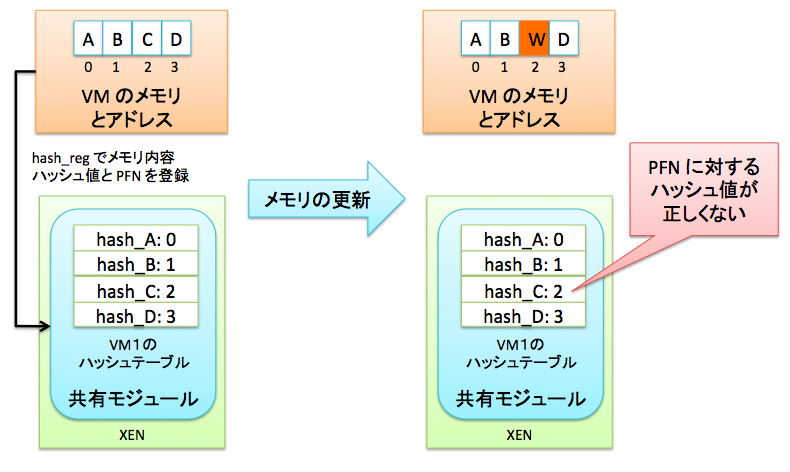
\includegraphics[width=10.0cm]{./img/non-renewal.png}\caption{ メモリの更新とハッシュテーブル}\label{non-renewal}\end{center}\end{figure}

メモリのハッシュ値計算後からのメモリの更新の監視は XEN 上の LOG DIRTY SUPPORT 関数群を使用する.
この関数群では dirty ビットマップを用意して,メモリの更新を監視してくれる.
使用するに当たって,この関数群は既存のものであったため他の所でどのように使用されているかに
留意した.実際にこの関数は Live Migration の移送元での dirty を監視する時にしか使わないため
移送先で使用する分には問題なく使用できる.しかし,実際のソフトウェアとして使う場合は
移送しようとした時に毎回この関数群の dirty ビットマップが使用されてしまうため,dirty が追えなくなって
しまうので独自の dirty ビットマップを作成する必要があるだろう.
この関数群の仕組みとしては XEN 上に dirty ビットマップを置き,メモリの書き込みの
コードの部分に dirty ビットが立っていなかったら立てるという関数を埋め込み,
書き込み事にビットマップへマークするようになっている.
よってページの更新を確認したい時は dirty ビットマップのビットが立っているかを確認すれば良い.
この確認は paging\_mfn\_is\_dirty 関数で行える.
このように移送先でハッシュ値が一致した場合,ハッシュ値が正しいものであることを保証することによって
ハッシュ値の再計算を省き,オーバヘッドを減らした.
ここでは移送先でのハッシュ値の扱いについて説明をした.
次に移送元では登録後のハッシュ値の扱いをどのようにしていたかを説明する.
共有元でも hash\_reg でハッシュテーブルを作成後,メモリの内容が更新されても
ハッシュ値の再計算は行わない.そのため stage1 の非転送ページの候補を探す時に
ハッシュテーブルでハッシュ値が正しいものであるという保証はない.
しかし,共有する手順を考えてみると共有されているページに関してはハッシュ値が正しいものである
ことが保証されることがわかる.
まず hash\_reg により共有したい仮想マシン同士のハッシュテーブルを作成する.
その後 hash\_share 関数で共有する.hash\_share 関数ではハッシュ値を比べて
一致した場合内容を確認して共有を行う.つまり移送元では共有の時点で
ESX と同様メモリの内容を確認して共有を行うためハッシュ値とメモリはこの時点では一致していると
考えることができる.
言いかえると共有されているメモリのハッシュ値は共有された時点では正しいことが保証されていることになる.
またメモリが更新される場合は共有が解かれることになるので共有されているページのハッシュ値は
保証されることになる.よって stage1 ではハッシュ値の再計算をせずに 
SharingMigration の処理を行うことができる.
このように原則 hash\_reg でハッシュテーブルにメモリ内容ハッシュ値を登録した後に
変更されたメモリは共有の対象としないことでハッシュ値の再計算を省きオーバヘッドを削減した.
またこの方法は本研究で共有の対象とするメモリが共有できなくなることはない.

stage3 では共有が実際に行えた PFN のリストを作成し移送元に送信する.

\subsubsection{STAGE4}
\label{sec-5-3-4}
stage4 では移送先で共有できたページを非転送ページとして設定する.
Live Migration のコードは XM ツールによりドメイン0のユーザランドで実行される.
XM ツールはハイパーコールなどを使用して,仮想マシンを Live Migration する.
そして XM が呼び出す Live Migration の中核となるプログラムが
XEN の操作ライブラリ XCLIB の一つの xc\_domain\_save.c である.
ドメイン0のユーザランドで Live Migration のコードを動かすのは XEN 上で行う場合,
TCP などソケットの扱いを初めから XEN のコードに記述しなくてはならなくなるため
Live Migration のコードがユーザランドで行われるのは当然の流れである.
このような場合は既存のドメイン0の OS の機能を使用する事で,XEN のコードはシンプルで肥大し過ぎないように
なっている.
SharingMigration は既存の Live Migration に追加する形で実装するため,
既存の Live Migration の仕組みに合わせた実装が必要になる.
xc\_domain\_save.c では pre-copy 方式の Live Migration が実装されている.
よって毎回のイテレートで送信するメモリのビットマップが用意されている.
つまりこのビットマップを上手く設定すれば非転送ページを設定することができる.
実際にはまず共有できたページのリストを移送先から受け取る.
ページリストを受け取ったら各ページが stage1-4 の間に書き換えられていなかったかを確認する.
この確認は xc\_shadow\_control 関数を用いて行う.
この関数は初期化のための呼び出しを行った後にこの関数が呼び出された時までのメモリページの
更新を監視するハイパーコール関数である.ハイパーコールの呼び出し後
XEN 上では移送元の stage2 で使用した LOG DIRTY SUPPORT 関数群を使用して
メモリの更新を監視している.
共有できたページが更新されていないか確認できたら,
xc\_domain\_save.c 上でページの送信を管理する
用に全てのビットが立った状態で用意されているビットマップの,そのページが対応するビットを落とす.
その様子を図 \ref{non-sending} に示す.
その後のイテレートフェーズではこのビットマップを参照して立っているビットを転送しようとするので
共有できたページを転送しないことができる.もちろん設定している最中にも
メモリは更新される場合がある.なので stage4 の最中もメモリの dirty は監視しており,
stage4 で更新ページ確認後更新されたページに関しては既存の Live Migration の
ファーストイテレートが終わった時点で再送すべきメモリページとして設定される.
移送先で共有されているページがもし移送元で更新されて再送することになっても
移送先では COW になっているページの上から内容を書き換えるだけなので問題なく動作する.

\begin{figure}[H]\begin{center}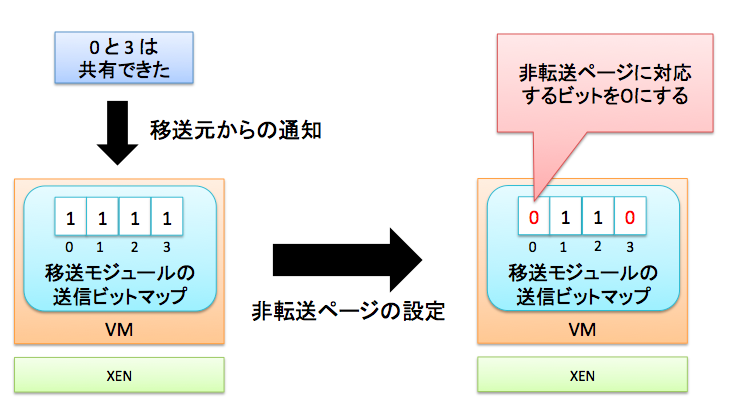
\includegraphics[width=10.0cm]{./img/non-sending.png}\caption{ 非転送ページの設定}\label{non-sending}\end{center}\end{figure}

\subsubsection{STAGE5}
\label{sec-5-3-5}
stage5 では sgage4 で設定された送信用のビットマップを初期の送信ビットマップとして
既存手法の pre-copy 方式 Live Migartion を行う.
このステージからは非転送ページを送らない設定以外は既存の手法と全く同じである.

\section{実験}
\label{sec-6}
本実験では既存手法より SharingMigration の方が PaaS 環境における
Live Migration において,移送時間が短く,CPU やネットワークの使用率も
削減することを示す.
実験環境を表 \ref{machine_env_host},\ref{machine_env_nfs} に示す.

\begin{table}[htb]
\caption{\label{machine_env_host}実験環境(ホストマシン)}
\centering
\begin{tabular}{|l|l|}
\hline
 & ホストマシン\\
 & (移送先,移送元)\\
\hline
OS & Ubuntu 14.04 LTS\\
\hline
メモリ & 4GB\\
\hline
CPU & Intel(R) Xeon(R) CPU X5650  @ 2.67GHz\\
\hline
NETWORK & Gigbit Ethernet\\
\hline
VMM & XEN 4.3.3-rc1\\
\hline
\end{tabular}
\end{table}

\begin{table}[htb]
\caption{\label{machine_env_nfs}実験環境(NSF サーバ)}
\centering
\begin{tabular}{|l|l|}
\hline
 & NFS サーバ\\
\hline
OS & Ubuntu 14.04 LTS\\
\hline
メモリ & 15GB\\
\hline
CPU & Intel(R) Xeon(R) CPU X3480  @ 3.07GHz\\
\hline
NETWORK & Gigbit Ethernet\\
\hline
VMM & XEN 4.3.3-rc1\\
\hline
\end{tabular}
\end{table}

なお比較対象は XEN に実装されている既存の Pre-copy を用いた
Live Migration とする.
\subsection{非転送ページの量を調整した本実装の実験}
\label{sec-6-1}
\subsubsection{目的}
\label{sec-6-1-1}
SharingMigration は移送する仮想マシンが持つ移送先でも共有可能で非転送可能なページを
対象に移送ページを削減する.
この実験では移送する仮想マシンと移送先にある仮想マシンに故意的に同様のメモリページを
持たせて,その量を変更することで非転送ページの量を調整し,移送時間を測定する.
この実験で既存手法より SharingMigration の方が非転送ページの量に応じて
移送時間が削減され,CPU やネットワークの使用率を削減できることを示す.

\subsubsection{実験方法}
\label{sec-6-1-2}
実験のマシン配置を図 \ref{exp01_arrangement} に示す.
まず稼働する仮想マシンは3つで移送元に2つ,移送先に1つである.
全ての仮想マシンの OS は Ubuntu 14.04.1 LTS を使用する.
それぞれの仮想マシンのメモリ容量は 512MB で,各仮想マシンの仮想ディスクは
NFS により同じネットワーク内の異なるマシンに配置する.
各仮想マシンには PaaS 環境を想定して,共通のメモリページを持たせる.
方法としては,ランダムな数字で埋められた同様のファイルを mmap で
各仮想マシンのメモリに書き込ませる.
この書き込む量を調整することで各仮想マシンが共通して持つメモリページ量を
調整する.
VM のワークロードは mmap のみで,書き込みの多いワークロードや読み込みを必要とする
ワークロードは基本的には動かさない.
全ての仮想マシンに同様のメモリを持たせたところで
移送元マシンの共有可能なメモリを共有する.また移送先では
VM3 のメモリをハッシュテーブルに登録しておく.
その後, VM2 を SharingMigration する.

なお,今回の実験では既存の Live Migration と比較を行うため,
仮想マシン間のメモリの共有までは同様に行うがその後に SharingMigration をせず
既存の Live Migration を行うものも結果に含めてある.

\begin{figure}[H]\begin{center}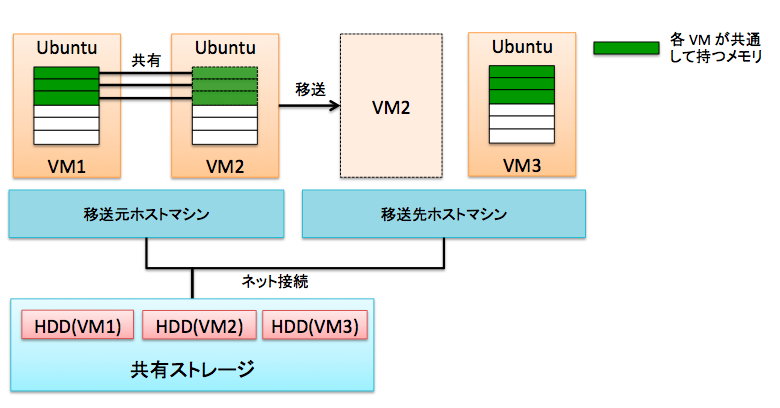
\includegraphics[width=12.0cm]{./img/exp01_arrangement.png}\caption{ 実験のマシン配置図}\label{exp01_arrangement}\end{center}\end{figure}

\subsubsection{実験結果}
\label{sec-6-1-3}
実験結果を図 \ref{exp_result} に示す.
X 軸が非転送ページの量,Y 軸が時間 [msec] である.
時間の内訳は,Live Migration の最初のイテレートが first iterate, それ以降のイテレート時間総和が
ohter iterate,SharingMigration のために追加実装したモジュールにかかった時間を module time,
それ以外の TCP のコネクションなど諸設定にかかった時間が other である.
また非転送ページ数が1以上のものが SharingMigration を行った実験結果で,
0のものが既存の Live Migration である.

結果として,非転送ページが多い程移送時間が短いことがわかった.
移送時間は最大 37 \% 削減することができた.
最初の送信量が削減されているので first iterate の時間が短くなっていることがわかる.
その後のイテレートに関しては今回のワークロードでは書き込みが行われないので,
ほぼ同じ時間となった.また非転送ページが増えるほど,移送先での共有などの処理が増えるので
モジュールの時間は非転送ページが多くなる程比例して大きくなることがわかる.
これらの結果は非転送ページ分移送量が減るので移送時間が短くなる妥当な結果といえる.
この結果から移送する仮想マシンが移送先で共有できるページを持っている場合は
そのページを移送先で共有して送信しないことで送信メモリ量を削減できることがわかった.
送信メモリ量が削減できることでネットワークの使用率が下がり,
移送時間が削減されることで CPU の使用時間も少なくなり
移送するマシン以外の仮想マシンへの影響を軽減することができることが考えられる.

\begin{figure}[H]\begin{center}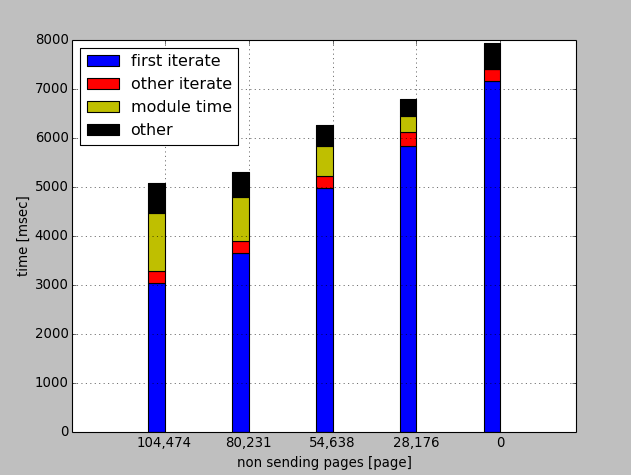
\includegraphics[width=8.0cm]{./img/exp_result.png}\caption{ 実験結果}\label{exp_result}\end{center}\end{figure}

\clearpage
\subsection{計測方法}
\label{sec-6-2}
\subsubsection{各マシンでのコマンドの実行方法}
\label{sec-6-2-1}
実験をするために Python によるスクリプトを書いた.
本研究の実験では各仮想マシン,ホストマシン上でスクリプトを起動させる必要がある.
また各マシン上で稼働させるスクリプトは同期をとり,タイミングを合わせなければならない.
この場合,1台のホストマシンから各マシン上でコマンドを実行できれば上記の問題は解決すると
考えられる.
しかし本研究では仮想マシンは完全仮想化を用いるため,ホストマシンのコマンドプロンプトから
直接アクセスすることができない.また,異なるホストマシン上で直接コマンドを実行させることもできない.
そこで今回は Python の paramiko モジュールを利用した.
paramiko モジュールは ssh を使用した,リモートコマンド実行ツールである.
よって各ホストマシン,完全仮想化された各仮想マシンで ssh を導入すれば一台のマシンから
各マシン上でコマンドを実行することができる.
このモジュールの使用方法をソースコード \ref{paramiko} に示す.
まずクライアントとなるクラスインスタンスを作成し,
次に,このクラスを初期化しクラスメソッドの connect を呼び出して,
リモート接続先と繋げる.connect の第二引数は接続先 ssh のポート番号である.
最後に実行したいコマンドを exec\_command メソッドで実行する.
\begin{lstlisting}[language=Python, caption=paramikoの使用法, label=paramiko]
# クライアントのクラスインスタンスを生成
client = paramiko.SSHClient()

# クラスインスタンスの初期化
client.set_missing_host_key_policy(paramiko.AutoAddPolicy())

# クライアントとコマンド実行先を繋げる
client.connect("hostname", 22, "username", "password")

# 実行したいコマンドを実行
client.exec_command("実行コマンド")
                         
\end{lstlisting}
\ \newline

paramiko には2つ問題がある.
まず一つ目の問題はセキュリティ面である.このコードでもわかるように
接続先との接続ではソースコードに,ユーザネームとパスワードまで書き込まなければならない.
つまりファイルを暗号化したりするなど対策を取らないと,ユーザネームとパスワードの
セットをそのまま置いとくことになり脆弱性に繋がる.
今回の実験ではアクセスするマシンで重要な機密は扱っていないため paramiko モジュールを
用いている.
二つ目が接続先でのコマンドの実行の方法である.
paramiko は接続先で シェルを使用してコマンドを実行する.
このとき実行方法はシェルプロセスを毎回作成し,そのプロセスに指定した実行コマンドを
行わせる.つまり実行コマンド間でのプロセス親子関係はなく,前に行ったコマンドを wait することなどが
できない.
実験スクリプトを書くとき,コマンドがまだ終わっていないのに次のコマンドを実行されると
都合が悪い.そこで苦肉の策として,実行コマンドの毎回の出力を全て読み取るようにした.
そうすることで実行コマンドが終わるまで待つことができる.
このように本実験では paramiko を使ったリモートコマンド実行により各マシン上でコマンドを実行する.
それによって,マシン間の同期をとりながら実験のコマンドを実行することができる.

\subsubsection{時間の測定方法}
\label{sec-6-2-2}
時間の測定方法はソースコード内に,指定したファイルにその時の時間と
どのフェーズかのフェーズ名を書き込むことによって測定する.
それを最後のパースフェーズでパースすることによって
測定したい時間を求める.このときコードを追加する場所は大きく二つに
わけられる.
一つ目が XM ツールの python コードである.
これは主に XM の migrate コマンド開始時から終了までの時間を測定するためである.
時間の測定には time モジュールの time メソッドを用いる.
これは gettimeofday と同様に UTC におけるエポックからの秒数を返す.
gettimeofday と異なる点は単位で,gettimeofday はマイクロ秒の値を返すのに対して
time.time() では小数点第六位まである秒で返す.つまり測っている時間は同じである.
もし gettimeofday が実装されている場合は,この関数は gettimeofday を使用する.
二つ目が xc\_domain\_save.c と xc\_domain\_resotore.c である.
xc\_domain\_save が移送元,xc\_domain\_restore が移送先で実行される Live Migration の
コードである. コードは C 言語なので測定をしたい箇所に gettimeofday を書き込む.
時間を表示するようにしたら測定したい場所同士の時間を引き算することで
その間の時間が求まる.

\subsubsection{実験スクリプトの流れ}
\label{sec-6-2-3}
実験スクリプトの大まかな流れをソースコード \ref{exp_code} に疑似コードとして
示す.可読性をあげるために
移送元ホストマシンでこのスクリプトを実行するのだが対応が分かり易くなる様に移送元ホストマシンにも
paramiko でリモートコマンドを実行するような書き方になっている.
また移送元,移送先どちらのホストマシンでも行うコマンドについてはマクロを定義した.

疑似コードについて説明をする.まず paramiko により移送元,移送先とのリモートコマンド実行用の
インスタンスを生成する.
次に initialize\_log\_files() でログファイルを全て消す.このログファイルは時間を測定するために用意されたもので
前の実験の値が書き込まれている.実験中これらのファイルに測定された時間が書き込まれる.
create\_domU クラスではホスト上で必要な仮想マシン(domU)を稼働させ,それを管理しているインスタンスを返す.
そして wait\_startup 関数でそれぞれの仮想マシンが完全に起動するまで待つ.
この確認方法は paramiko を用いた,仮想マシンへの ssh アクセスを元に行っている.
もし paramiko で ssh アクセスが行えたら起動したと判断することができる.
exec\_script 関数では仮想マシンで実行したいスクリプトを読み込んで
各仮想マシン上で実行する.
次にベンチマークを動かす場合はベンチマークをベンチマーク専用のマシン上で実行させる.
これはベンチマークの稼働により実験ホストマシンの CPU などが使われないためである.
そして enable\_share 関数で仮想マシンのページ共有のための初期化を行う.
初期化後,これより前の実験で利用した既に稼働していない domU のハッシュテーブルや
その他管理用に用意したデータを解放する.
この解放関数はハッシュテーブルを探索し,そのテーブルの仮想マシンがまだ
起動しているかを確認する.その時もし稼働していなかったらそれらのデータを解放するのだが,
関数呼び出しにシェアが可能となっている仮想マシンをトリガとして必要とする.
そのため,初期化にも関わらずこのような位置で行う.
その後,control\_module 関数で本提案のモジュールの ON か OFF かを決める.
そして hash\_reg で各仮想マシンのハッシュテーブルを作成し, hash\_sahre 関数で
ハッシュテーブルを用いてメモリを共有する.
共有が完了したら SharingMigration を開始する.
しかしその前にハッシュテーブル作成やメモリ共有のために使われたキャッシュを
ベンチマークに使用させなければ,実際の環境を再現できないので十分な時間待つことが必要となる.
最後に測定時間を書き込んだファイルを移送先から読み込み,自分のはローカルから読み込み,
それらを解析することで時間が測定できる.

\clearpage
\begin{lstlisting}[language=Python, caption=実験の疑似コード, label=exp_code]
# 移送元と移送先の paramiko の接続
src_host = paramiko.connect("source_host")
dst_host = paramiko.connect("destination_host")

# コードを簡略化するためマクロ定義
MACRO hosts.XXX() => {src_host.XXX() ; dst_host.XXX()}

# LOG ファイルを初期化
hosts.initialize_log_files()

# 必要な台数の仮想マシンを起動
src_domU = src_host.create_domU()
dst_domU = dst_host.create_domU()
hosts.wait_startup()

# 各仮想マシン上で任意のスクリプトを実行する
src_domU.exec_script("source_script")
dst_domU.exec_script("destination_script")

# ベンチマークを起動する場合ここで実行
if BENCHMARK :
   bench_host = paramiko.connect("bench_host")
   bench_host.start_bench()
   
# domU のページ共有を可能にし
# ホストマシンの管理するハッシュテーブルの初期化
hosts.enable_sahre()
hosts.initialize_hash_tables()

# 本提案のモジュールのスイッチ
if MODULE:
   hosts.control_module("ON")
else:
   hosts.control_module("OFF")

# ハッシュテーブルの作成とハッシュテーブルを使用したページの共有
hosts.hash_reg()
hosts.hash_sahre()

# 移送
sleep(ENOUTH_TIME)
src_host.SharingMigrate(src_domU.get_migrate_vm(), "destination_host")

# LOG を解析
src_host.parse_log_files(dst_host)
                         
\end{lstlisting}

\clearpage
\section{おわりに}
\label{sec-7}
\subsection{まとめ}
\label{sec-7-1}
仮想化技術が様々な場面で使われており PaaS の提供なども
なされている.PaaS を提供する環境では同じ内容のメモリを多く持つ仮想マシンが複数存在する.
その環境内で Live Migration を行うと移送しなくて済むメモリの送信を行っている場合がある.
Live Migration 時には CPU やネットワークなどの資源を多く使用するため,
送らないで済むメモリを送信しなければ移送時間を減らし,資源の使用率も削減できる.

本研究では PaaS 環境における Live Migration で各仮想マシンが持つ共通のメモリページを
移送先で共有することで送信せず,転送メモリ量を減らす SharingMigration を提案した.
既存の Live Migration では移送先に共有可能で転送しなくても済むメモリページが
あったとしても全てのメモリページを送信していた.
結果,移送する仮想マシンが移送先でも共有できるメモリページを持っている場合,
メモリを送信せずに移送先で共有することでメモリ転送量を減らすことができる.
転送量削減により移送時間を削減し,使用する CPU 使用率も削減できる.
また転送量が減るのでネットワーク資源の占有量も減る.
よって他の仮想マシンへの影響も削減することができる.

\subsection{今後の課題}
\label{sec-7-2}
今回の実験でのワークロードは同様のファイルを mmap するというもので,
Live Migration 中には書き込みや読み取り処理を基本的には行わない.
基本的と書いたのは,OS の動作によるメモリ書き込みなどは行われるからである.
しかし,実際の PaaS 環境でユーザに提供されている仮想マシン上では
ユーザが様々なアプリケーションを稼働することが考えられる.
アプリケーションによっては,メモリ書き込みの激しいアプリケーションもある.
よって次の実験方針として,実践的なアプリケーション(特にメモリ書き込みを
多く行うもの)を用いた SharingMigraiton 実験が考えられる.
現在 memcached という分散型のメモリキャッシュシステムを用いた実験を進行中である.
memcached は大規模な Web サービスなどでよく用いられるアプリケーションで
ハードディスクなどの読み込みの遅いハードウェアを使用したデータベースなどから
読み込みをした場合,再び利用することを考慮してメモリ上にキャッシュするためのソフトウェアである.
memcached ではキャッシュする場合はメモリ書き込みを行い,読み取りの場合はメモリ読み出しを
行うので,ベンチマークでその量を調整し,書き込みの激しいワークロードも再現することができる.

また今回の実験では移送時間のみしか測定していない.
よって移送時間は削減できているが,短くなった移送時間内にかなりの CPU を消費している場合も
考えられる.よって今後の課題として CPU やネットワークの消費量も測定する必要がある.
測定には xentop コマンドを用いる.
この関数のソースコードでは様々な XEN 上の仮想マシンの状態を取得する関数が用意されている.
それらを使用し今後 CPU やネットワークの消費量を測定していく.

他にハードウェアの改善点についてもあげられる.
現在移送元マシンと移送先マシンと NFS サーバはローカルなネットワークで繋がっている.
もし memcached などのクライアントベンチマークを動かす場合はこのネットワークを
介してリクエストが投げられることになる.
よって Live Migration に使用するネットワーク上で memcached などのリクエストの
パケットも流さなくてはならないのでネットワークが混雑してしまう場合が想定される.
そこで図 \ref{nic} のようにホストマシン間に Live Migration の専用回線を繋げることで
ネットワークを確保することができる.

\begin{figure}[H]\begin{center}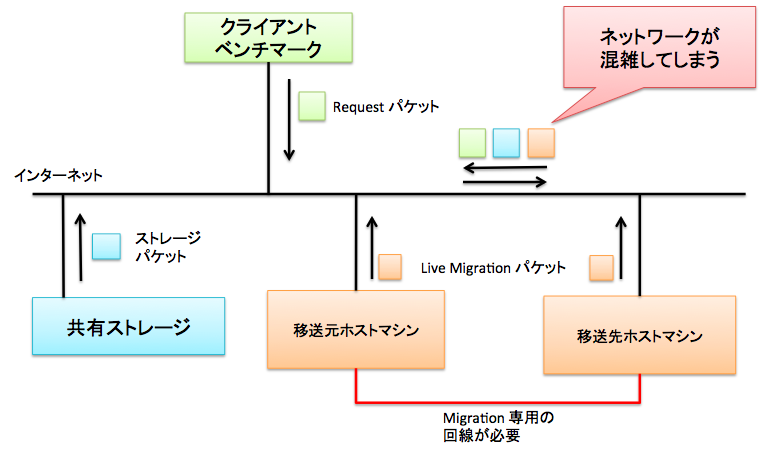
\includegraphics[width=10.0cm]{./img/nic.png}\caption{ マシン間回線}\label{nic}\end{center}\end{figure}

このようにネットワークを確保することで安定した実験を行うことができる.
仮想マシンの仮想ディスクとメモリを移送する VMware の Live Migration では
このように移送元と移送先ホストマシン間で Live Migration 専用の線を繋ぐように推奨している.
仮想ディスクの移送はメモリと比べて大きく時間を取るので安定した Live Migration を実現するためである.
今後仮想ディスクとメモリの Live Migration が主流になった場合このような
接続方法も必ずなされるようになる場合もあるのでこのような環境にした方がよいと考えられる.
また,現在の実験では仮想マシンのメモリは 512 MBであるが実際に扱う仮想マシンの
メモリはさらに大きい事が考えられる.Windows Azure\cite{azure} の Websites(PaaS) では
メモリ量はもう隠蔽されてしまっているのでわからないが,Azure の Virtual Machines インスタンスでは
最低のメモリ量が 768 MB となっている.よって将来的にもメモリ量は増加することが考えられるので
実験のメモリ量も増設すべきであると考えられる.


\clearpage
\section{謝辞}
\label{sec-8}
本研究を行うにあたり, 熱心にご指導頂いた河野健二准教授に心より御礼申し上げます. 
また, 最初から最後まで面倒を見て下さった古藤明音先輩にも深く感謝致します. 
最後に, 河野研究室の皆様からは様々なことを教えて頂きました. この場を借りて感謝致します.
\clearpage

\bibliographystyle{jplain}
\bibliography{ref}
% Emacs 24.5.1 (Org mode 8.2.10)
\end{document}
